\chapter{Results}
\label{chap:results}

This works goals were divided in basically two steps, initialization and
transmission (downlink). Having these two steps working it is possible to
understand and evaluate the results of such hardware platform. Figure
\ref{fig:setup} shows how the hardware is arranged. In Figure \ref{fig:setupbd}
it is possible to see the setup's block diagram, which gives the idea of the
complexity behind the design and how each component is connected, while Figure
\ref{fig:fpgaarea} reveals how much FPGA area this setup occupies, which implies
the complexity involved in the design.

%foto setup pronto
\begin{figure}[htbp]
    \centering
    \includegraphics[width=0.85\textwidth]{./figures/setup_pic}
    \caption{ Image of the setup hardware.
    \label{fig:setup}}
\end{figure}

%foto diagrama de blocos
\begin{figure}[htbp]
    \centering
    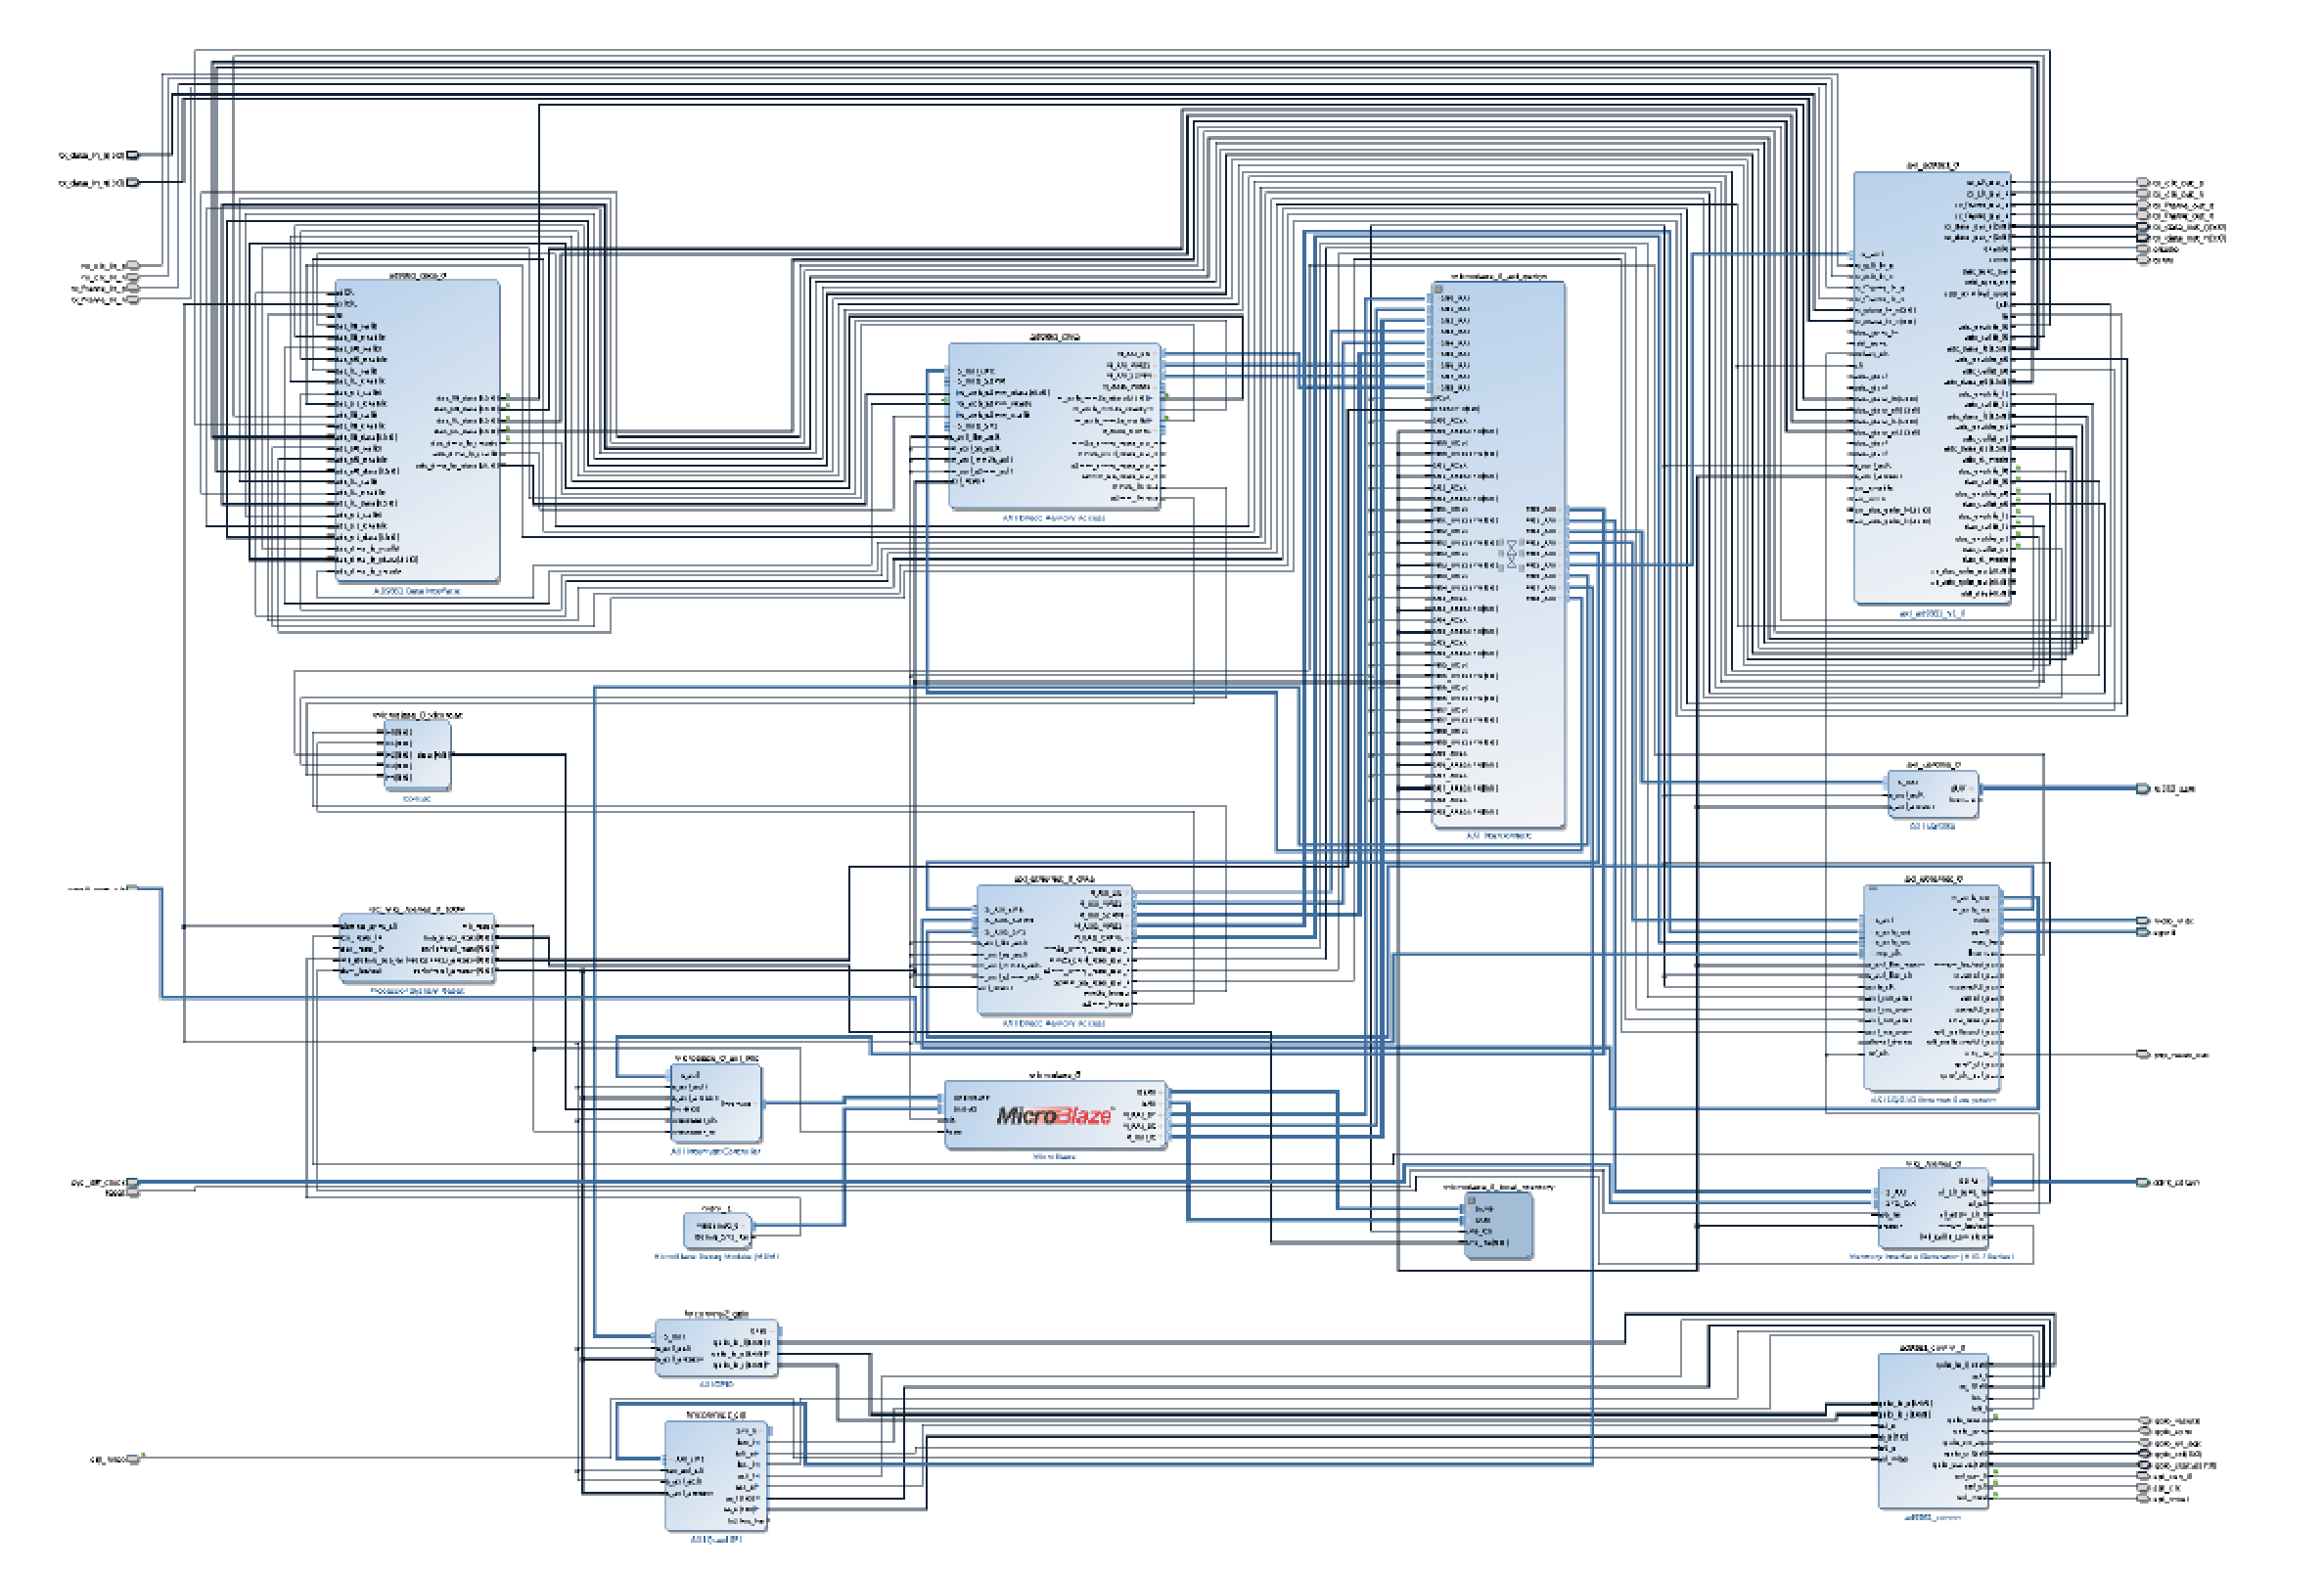
\includegraphics[width=0.95\textwidth]{./figures/setup_bd}
    \caption{ Image of the setup block diagram.
    \label{fig:setupbd}}
\end{figure}


\begin{figure}[htbp]
    \centering
    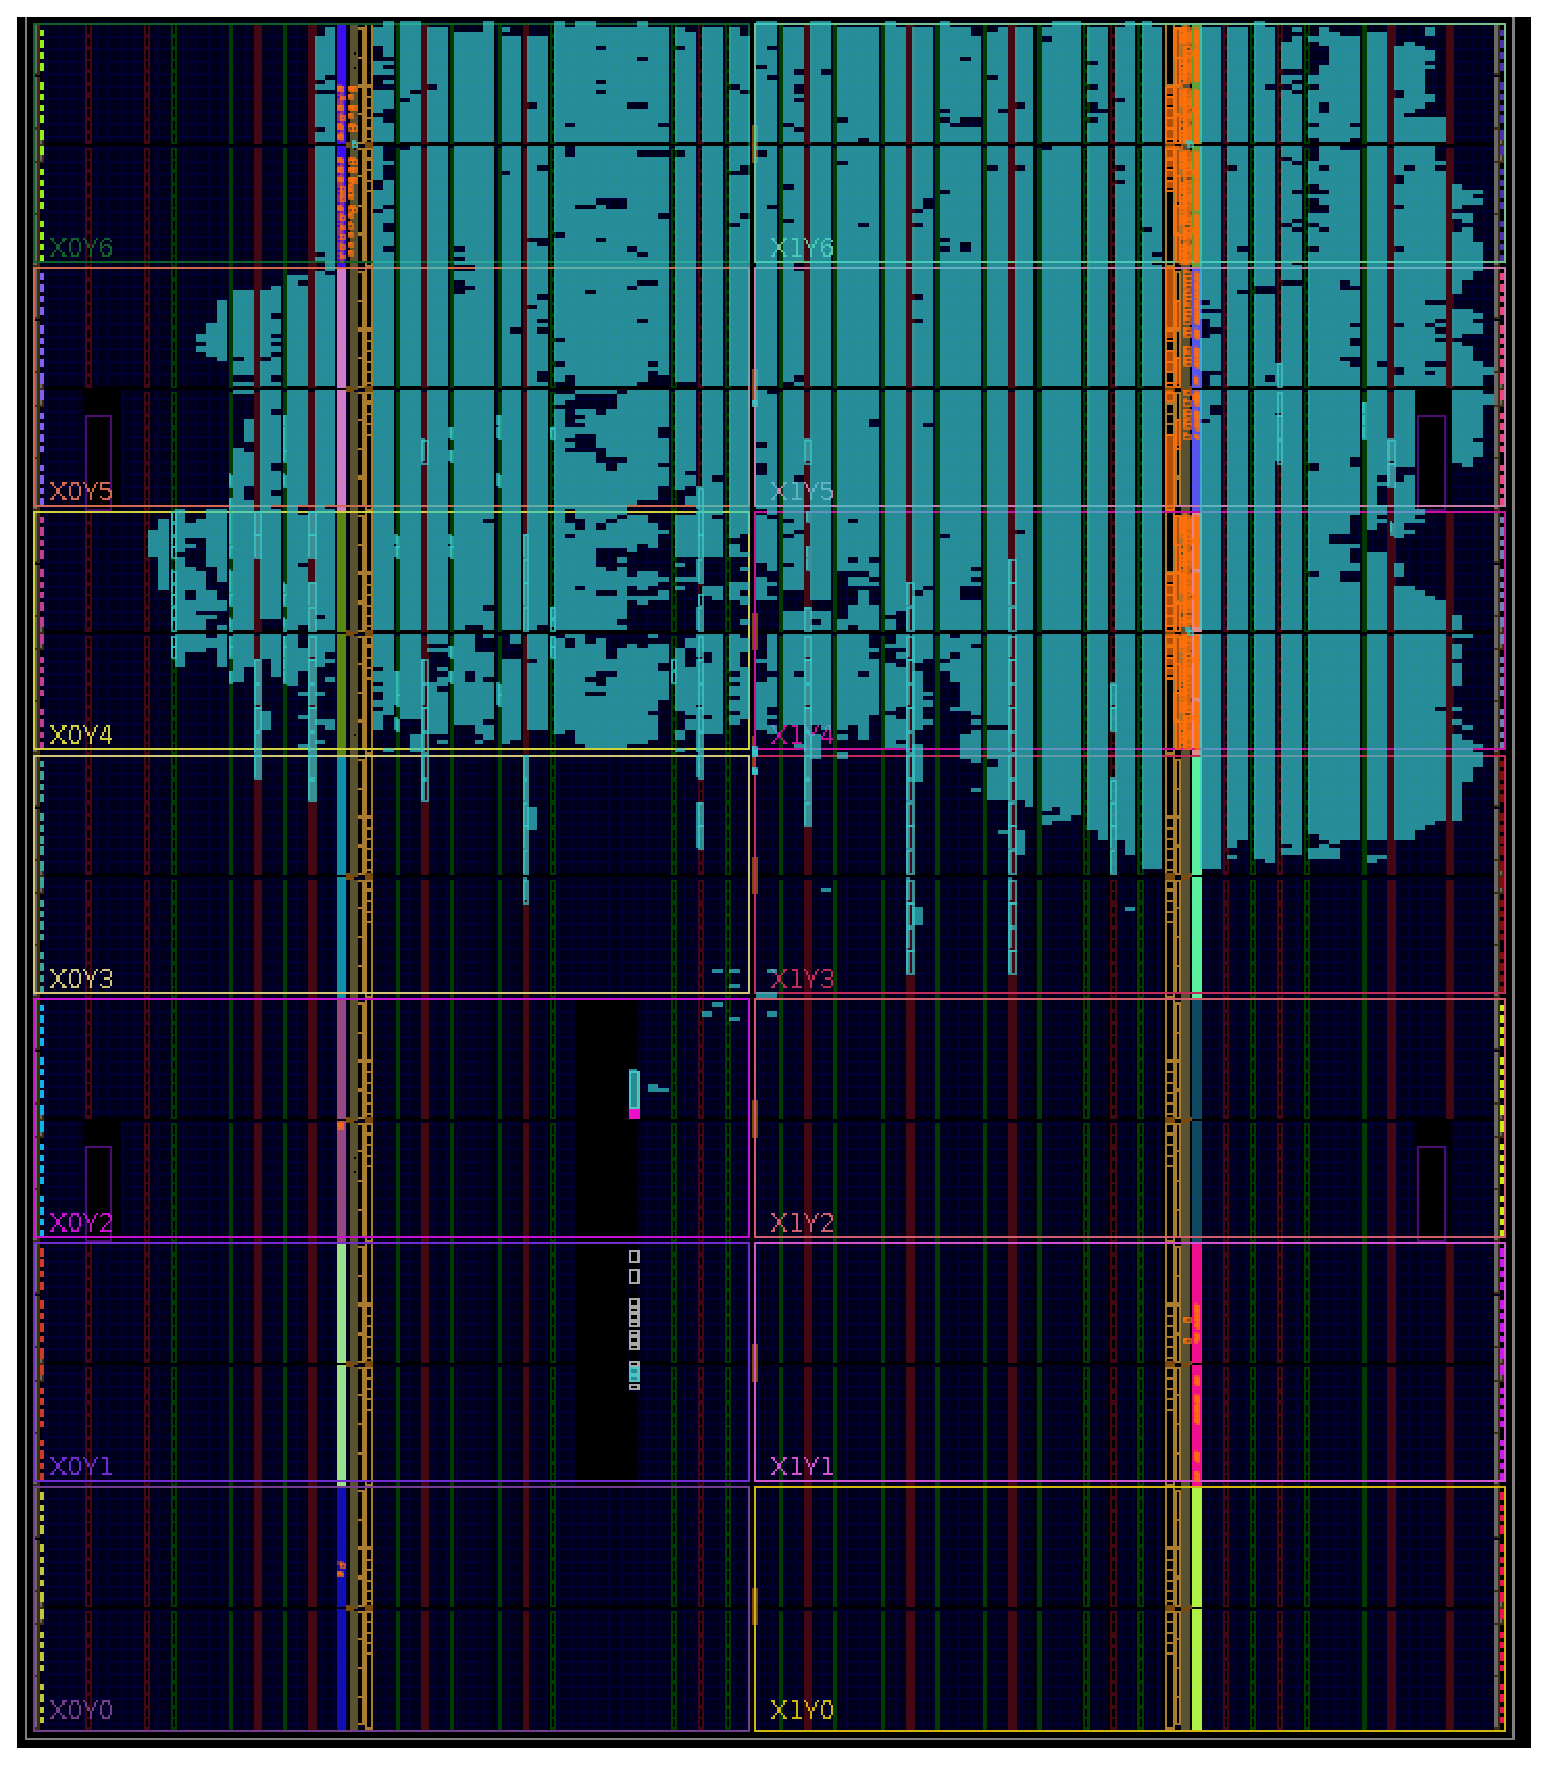
\includegraphics[width=0.35\textwidth]{./figures/fpga_area}
    \caption{ FPGA area used in this setup.
    \label{fig:fpgaarea}}
\end{figure}

\vfill
\clearpage

\section{Preliminary Tests}
\label{result:conf}

The preliminary tests focused on the initialization and communication between
FPGA and the FMComms2 board. In the previous chapter, the steps of setting up
communication and control interfaces were described, and it was particularly
stated that after the initialization and calibration is finished, it is possible
to observe the carrier wave centralized at the frequency 2.4 GHz.

To generate the outputs two analyzers were used, one mixed signal oscilloscope
(model MSO9104A) and one spectrum analyzer (model N9010A) both from Agilent
technologies company. In Figure \ref{fig:spec} it is possible to see the output
of the spectrum analyzer where the carrier wave is at 2.45 GHz and in Figure
\ref{fig:oscillfreq} there is the oscilloscope sinusoidal wave with frequency
measurements in the bottom of the picture.

%spectrum analyser image
\begin{figure}[htbp]
    \centering
    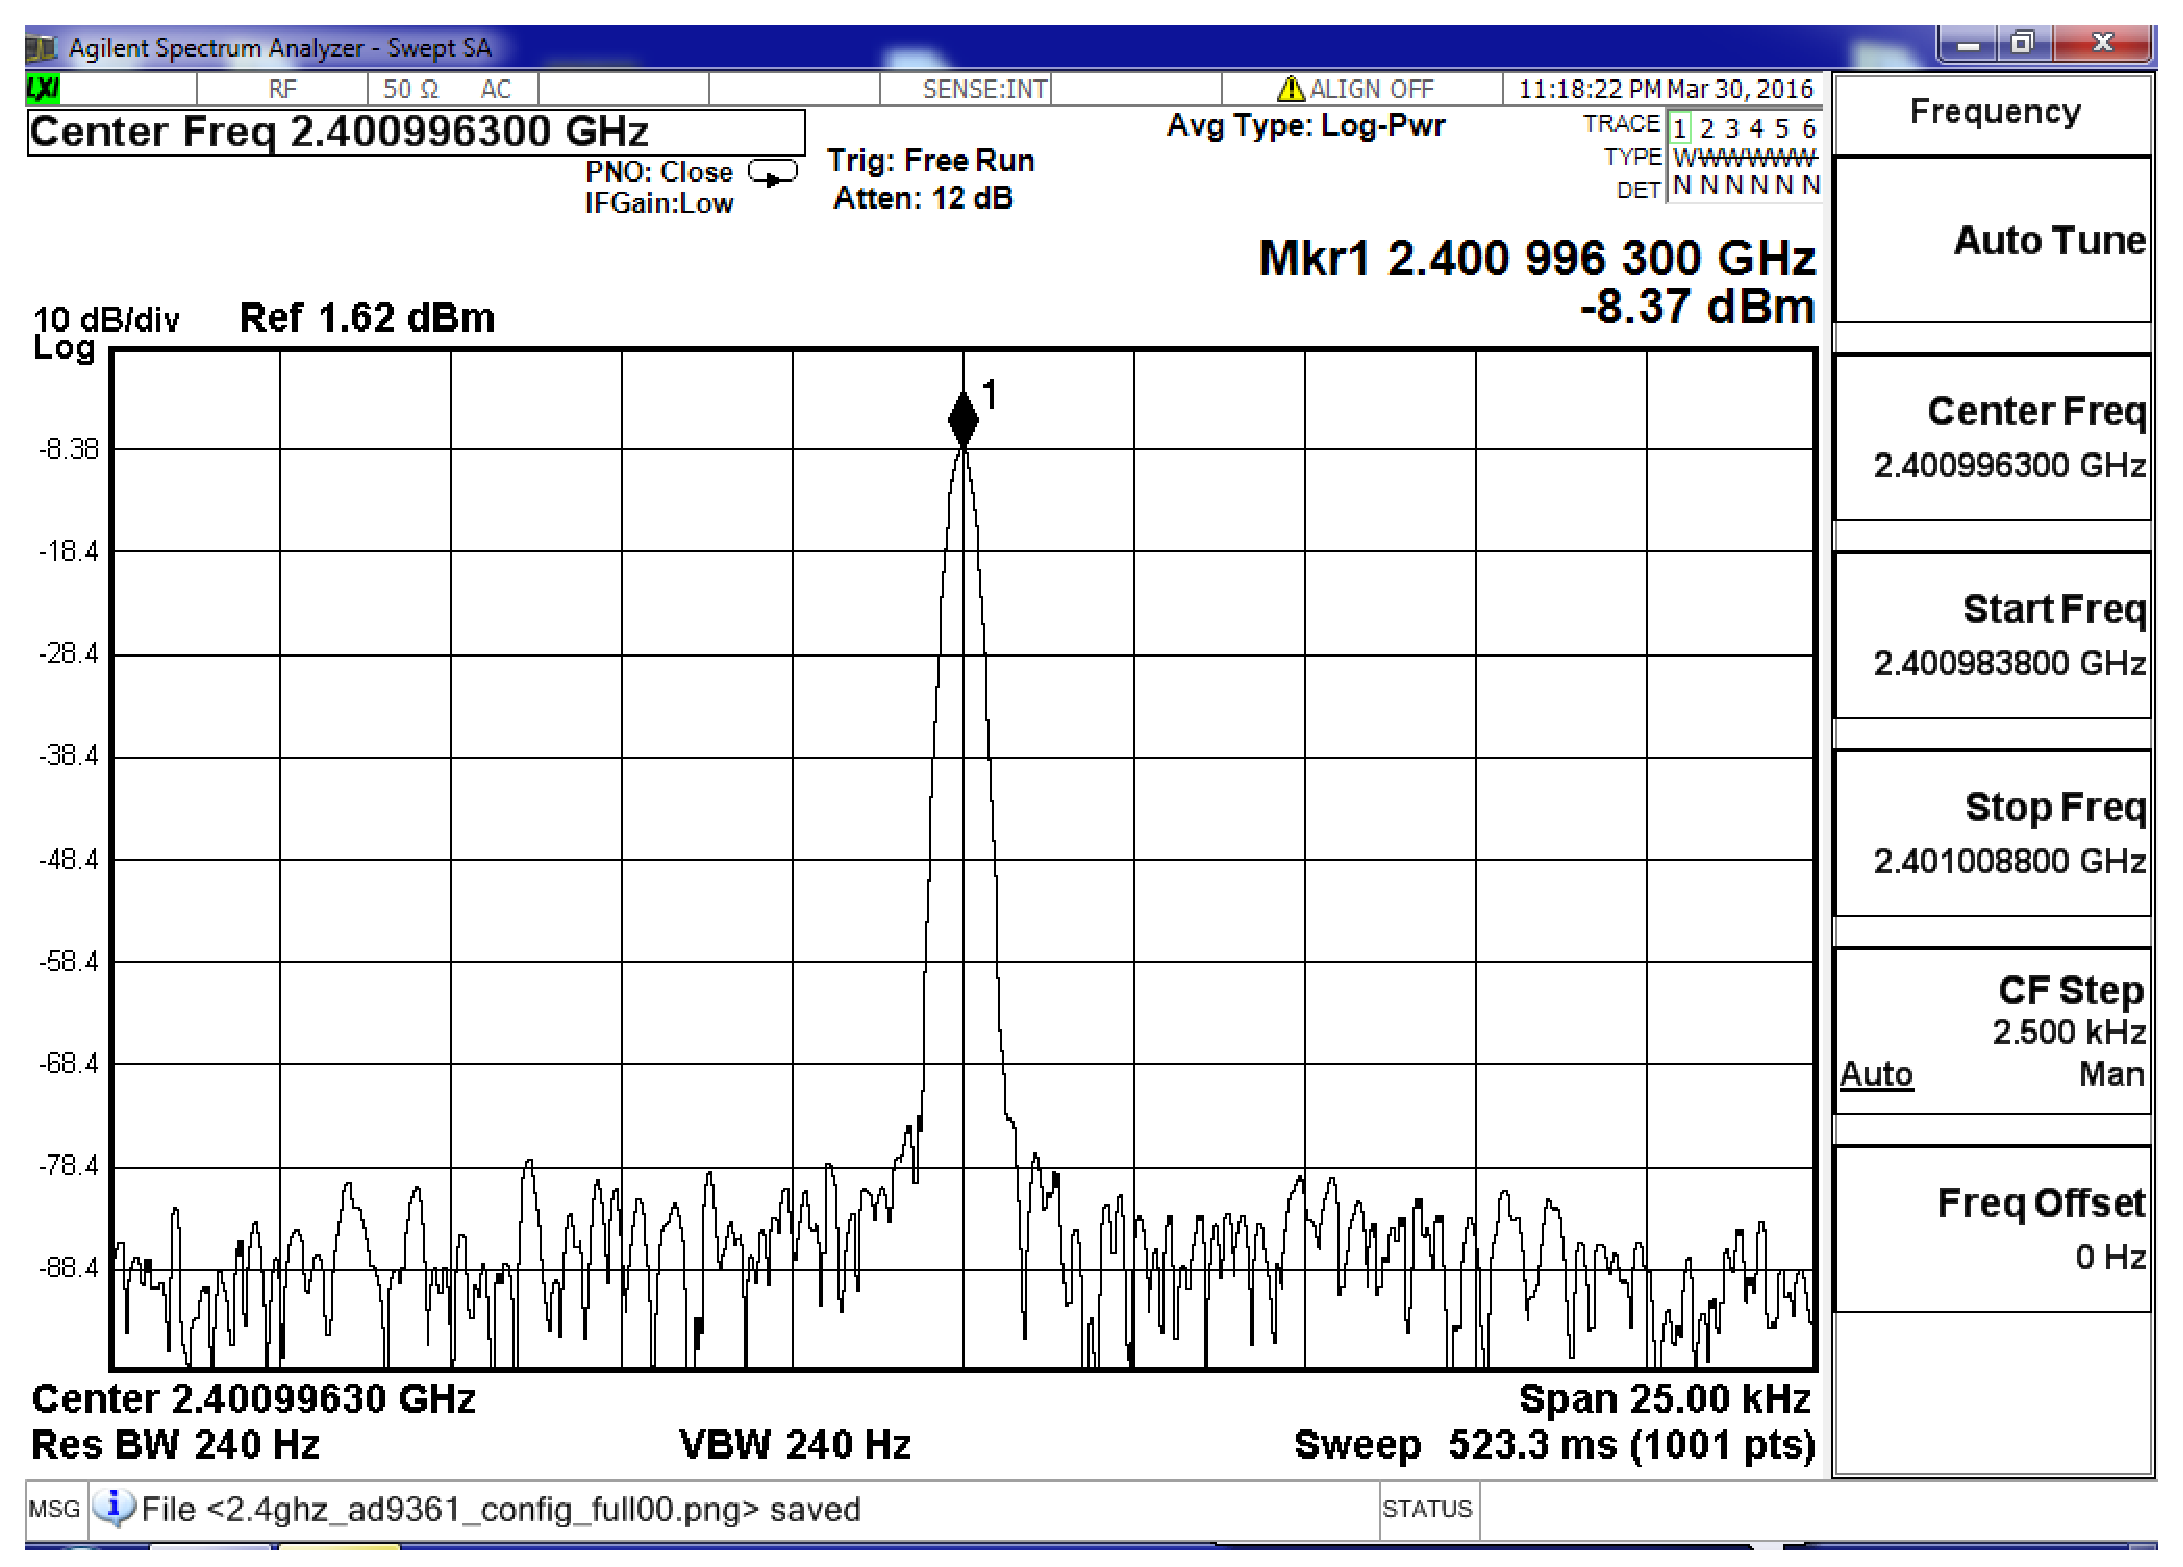
\includegraphics[width=0.85\textwidth]{./figures/spectrum_init}
    \caption{ Spectrum analyzer screen.
    \label{fig:spec}}
\end{figure}


%freq
\begin{figure}[htbp]
    \centering
    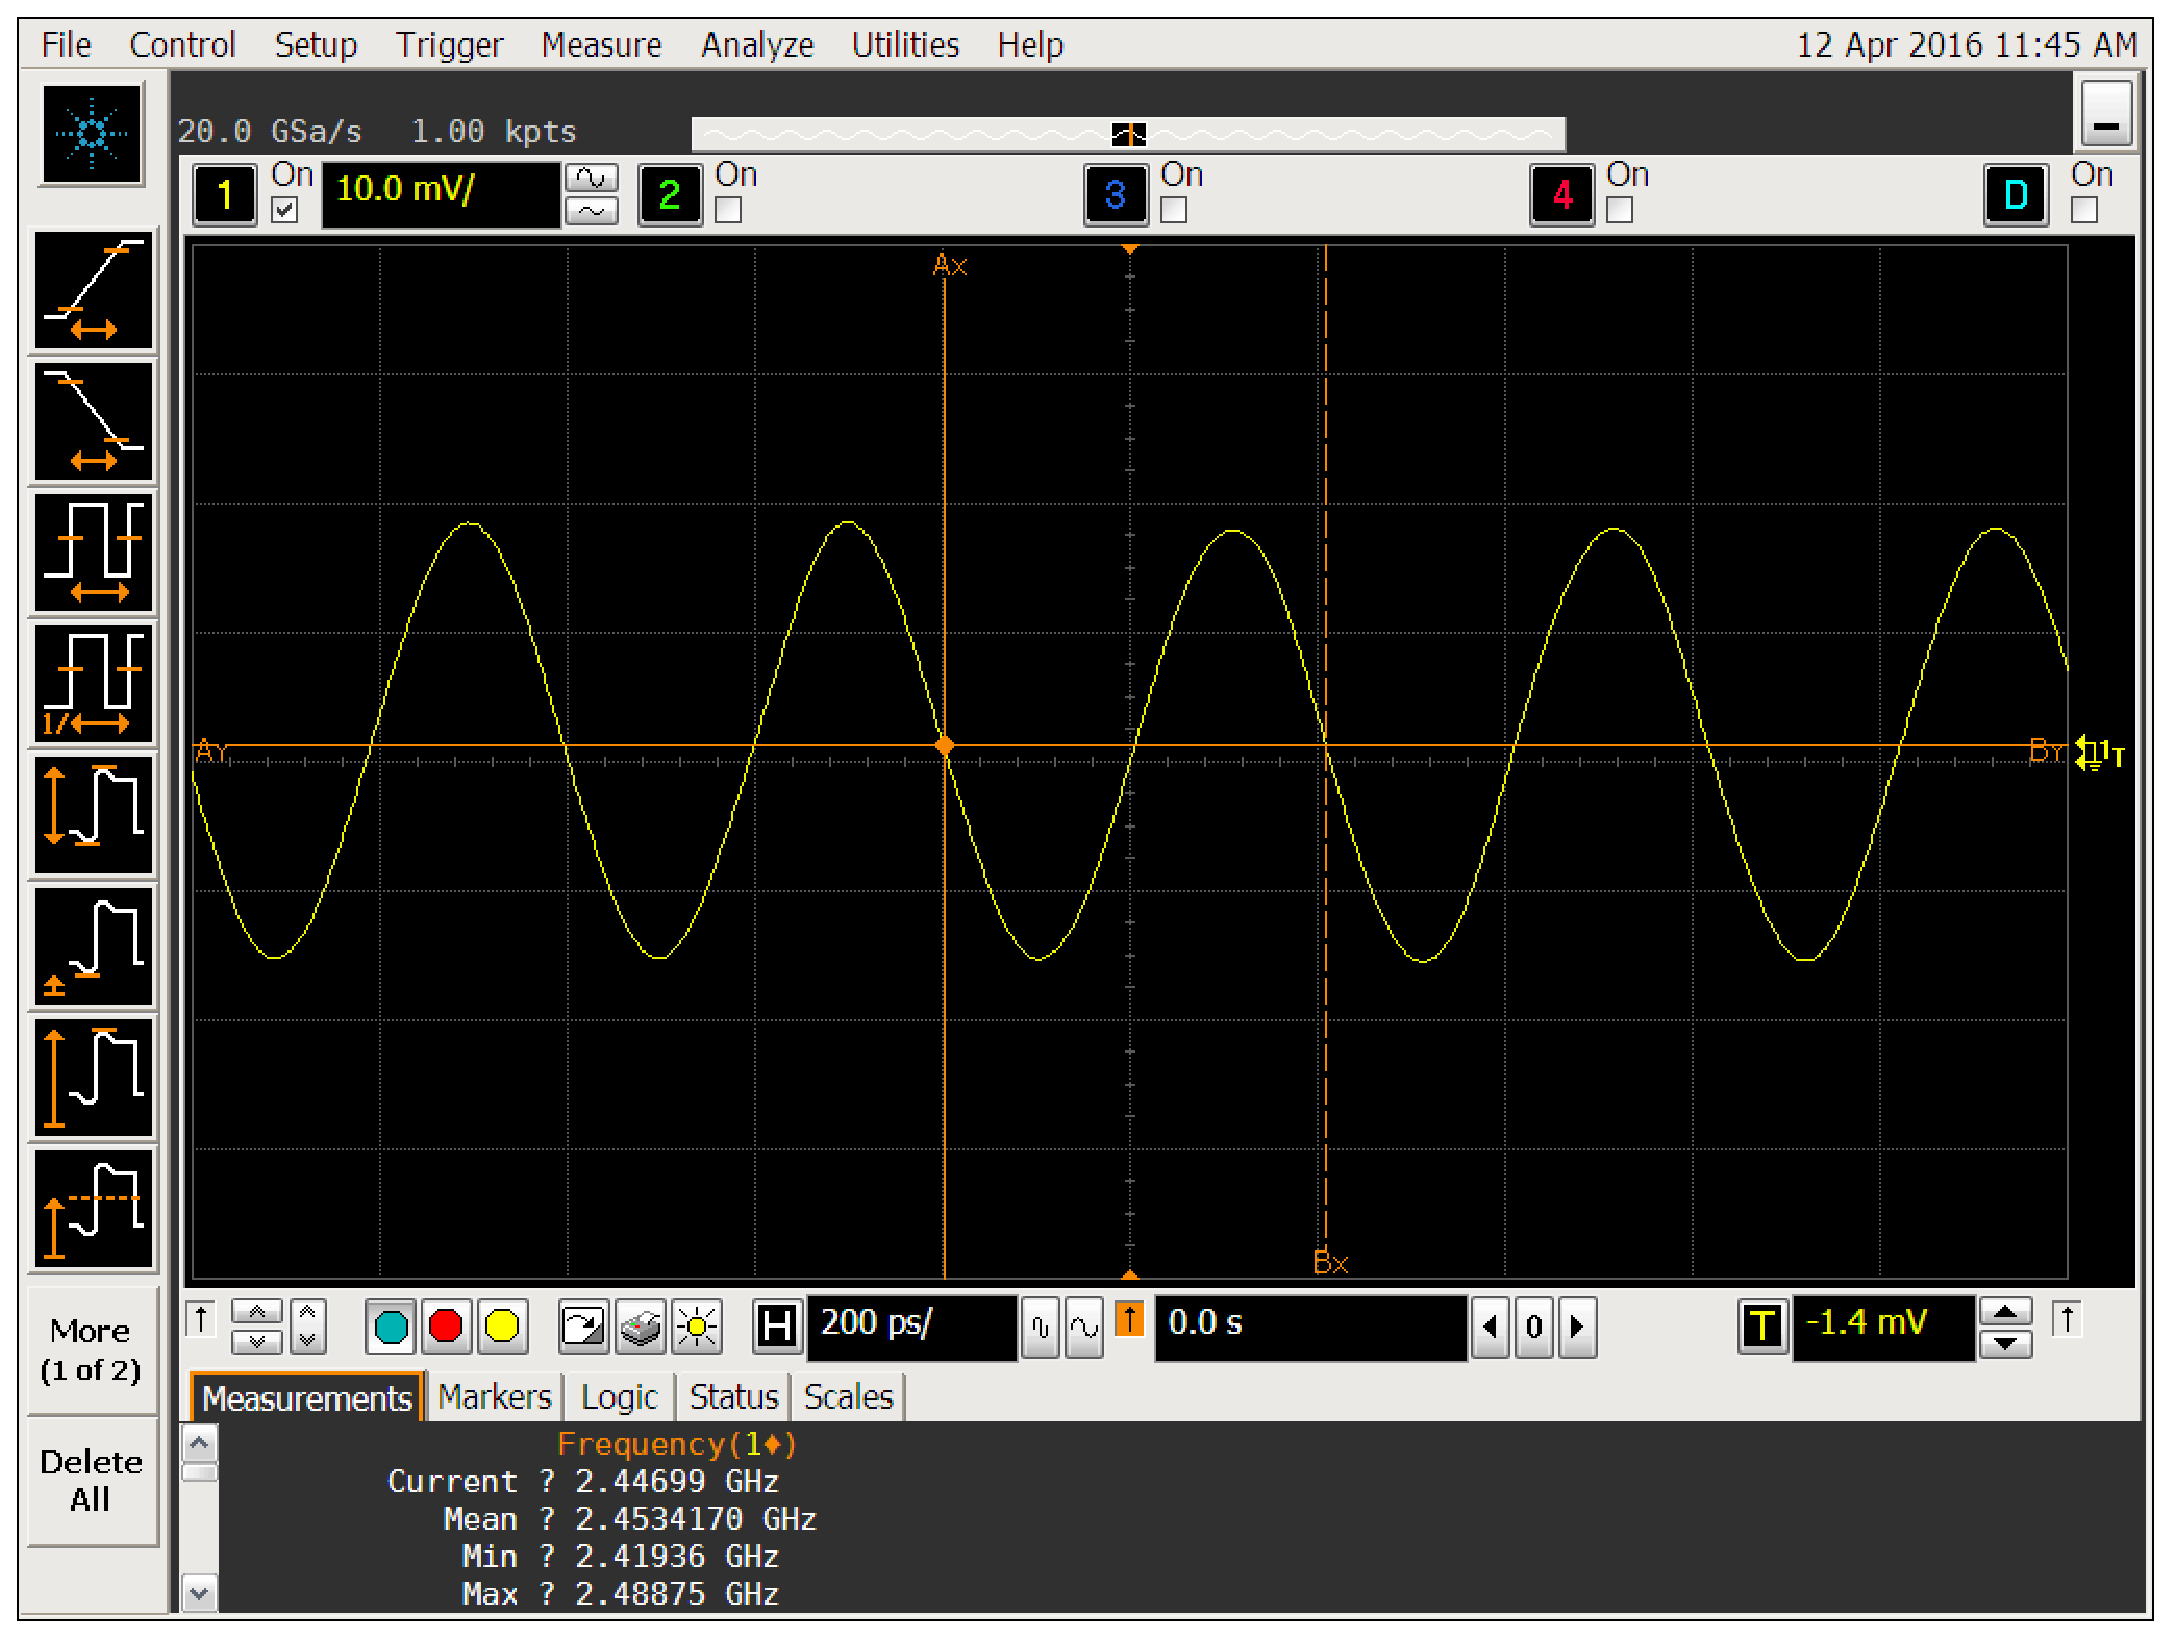
\includegraphics[width=0.85\textwidth,
    trim={{.17\textwidth} 0 {.02\textwidth} {.24\textwidth}},
    clip]{./figures/oscill_freq}
    \caption{ Carrier waveform with frequency Measurement.
    \label{fig:oscillfreq}}
\end{figure}


%\vfill
%\clearpage

\section{Simulation}

An important step in HDL development is the logic simulation of the circuit.
Through this simulation it is possible to monitor every port and be able to
understand the block behavior, thus correcting any problem or misbehavior.

\subsection{Transmit (DAC) Interface Simulation}

The simulation of the transmit interface, which interfaces the FPGA with DAC was
made in three steps. In the first step (Figure \ref{fig:simdacdma}) the DAC-DMA
Interface is simulated, in the second step (Figure \ref{fig:simdac}) the DAC
interface is simulated. Finally in the third step (Figure \ref{fig:simtxif}),
both of the interfaces are connected and the whole DAC chain is simulated. The
interface is composed by two blocks, there was the need to simulate each block
separately and sequentially simulate both blocks connected and working together,
in the Figures \ref{fig:simdacdma}, \ref{fig:simdac} and \ref{fig:simtxif} it is
possible to see the simulation results and wave diagrams of the three steps,
respectively.

In Figure \ref{fig:simdacdma}, it is possible to observe the behavior of the
\textit{dac-dmaIterface} block where the signal \textit{sig\_dma\_data} is fed
to the block, and the signals \textit{ sig\_axis\_axc0\_itdata,
sig\_axis\_axc0\_qtdata, sig\_axis\_axc1\_itdata and sig\_axis\_axc1\_qtdata}
are the \textit{IQ data} being fed to both to the \textit{dacInterface} block.
In this simulation the important point is to note that the 32 bits input signal
(\textbf{sig\_dma\_data}) is being divided in 16 bit streams (\textbf{
sig\_axis\_axc0\_itdata, sig\_axis\_axc0\_qtdata, sig\_axis\_axc1\_itdata and
sig\_axis\_axc1\_qtdata}) and being outputted by the block.

\begin{figure}[htbp]
    \centering
    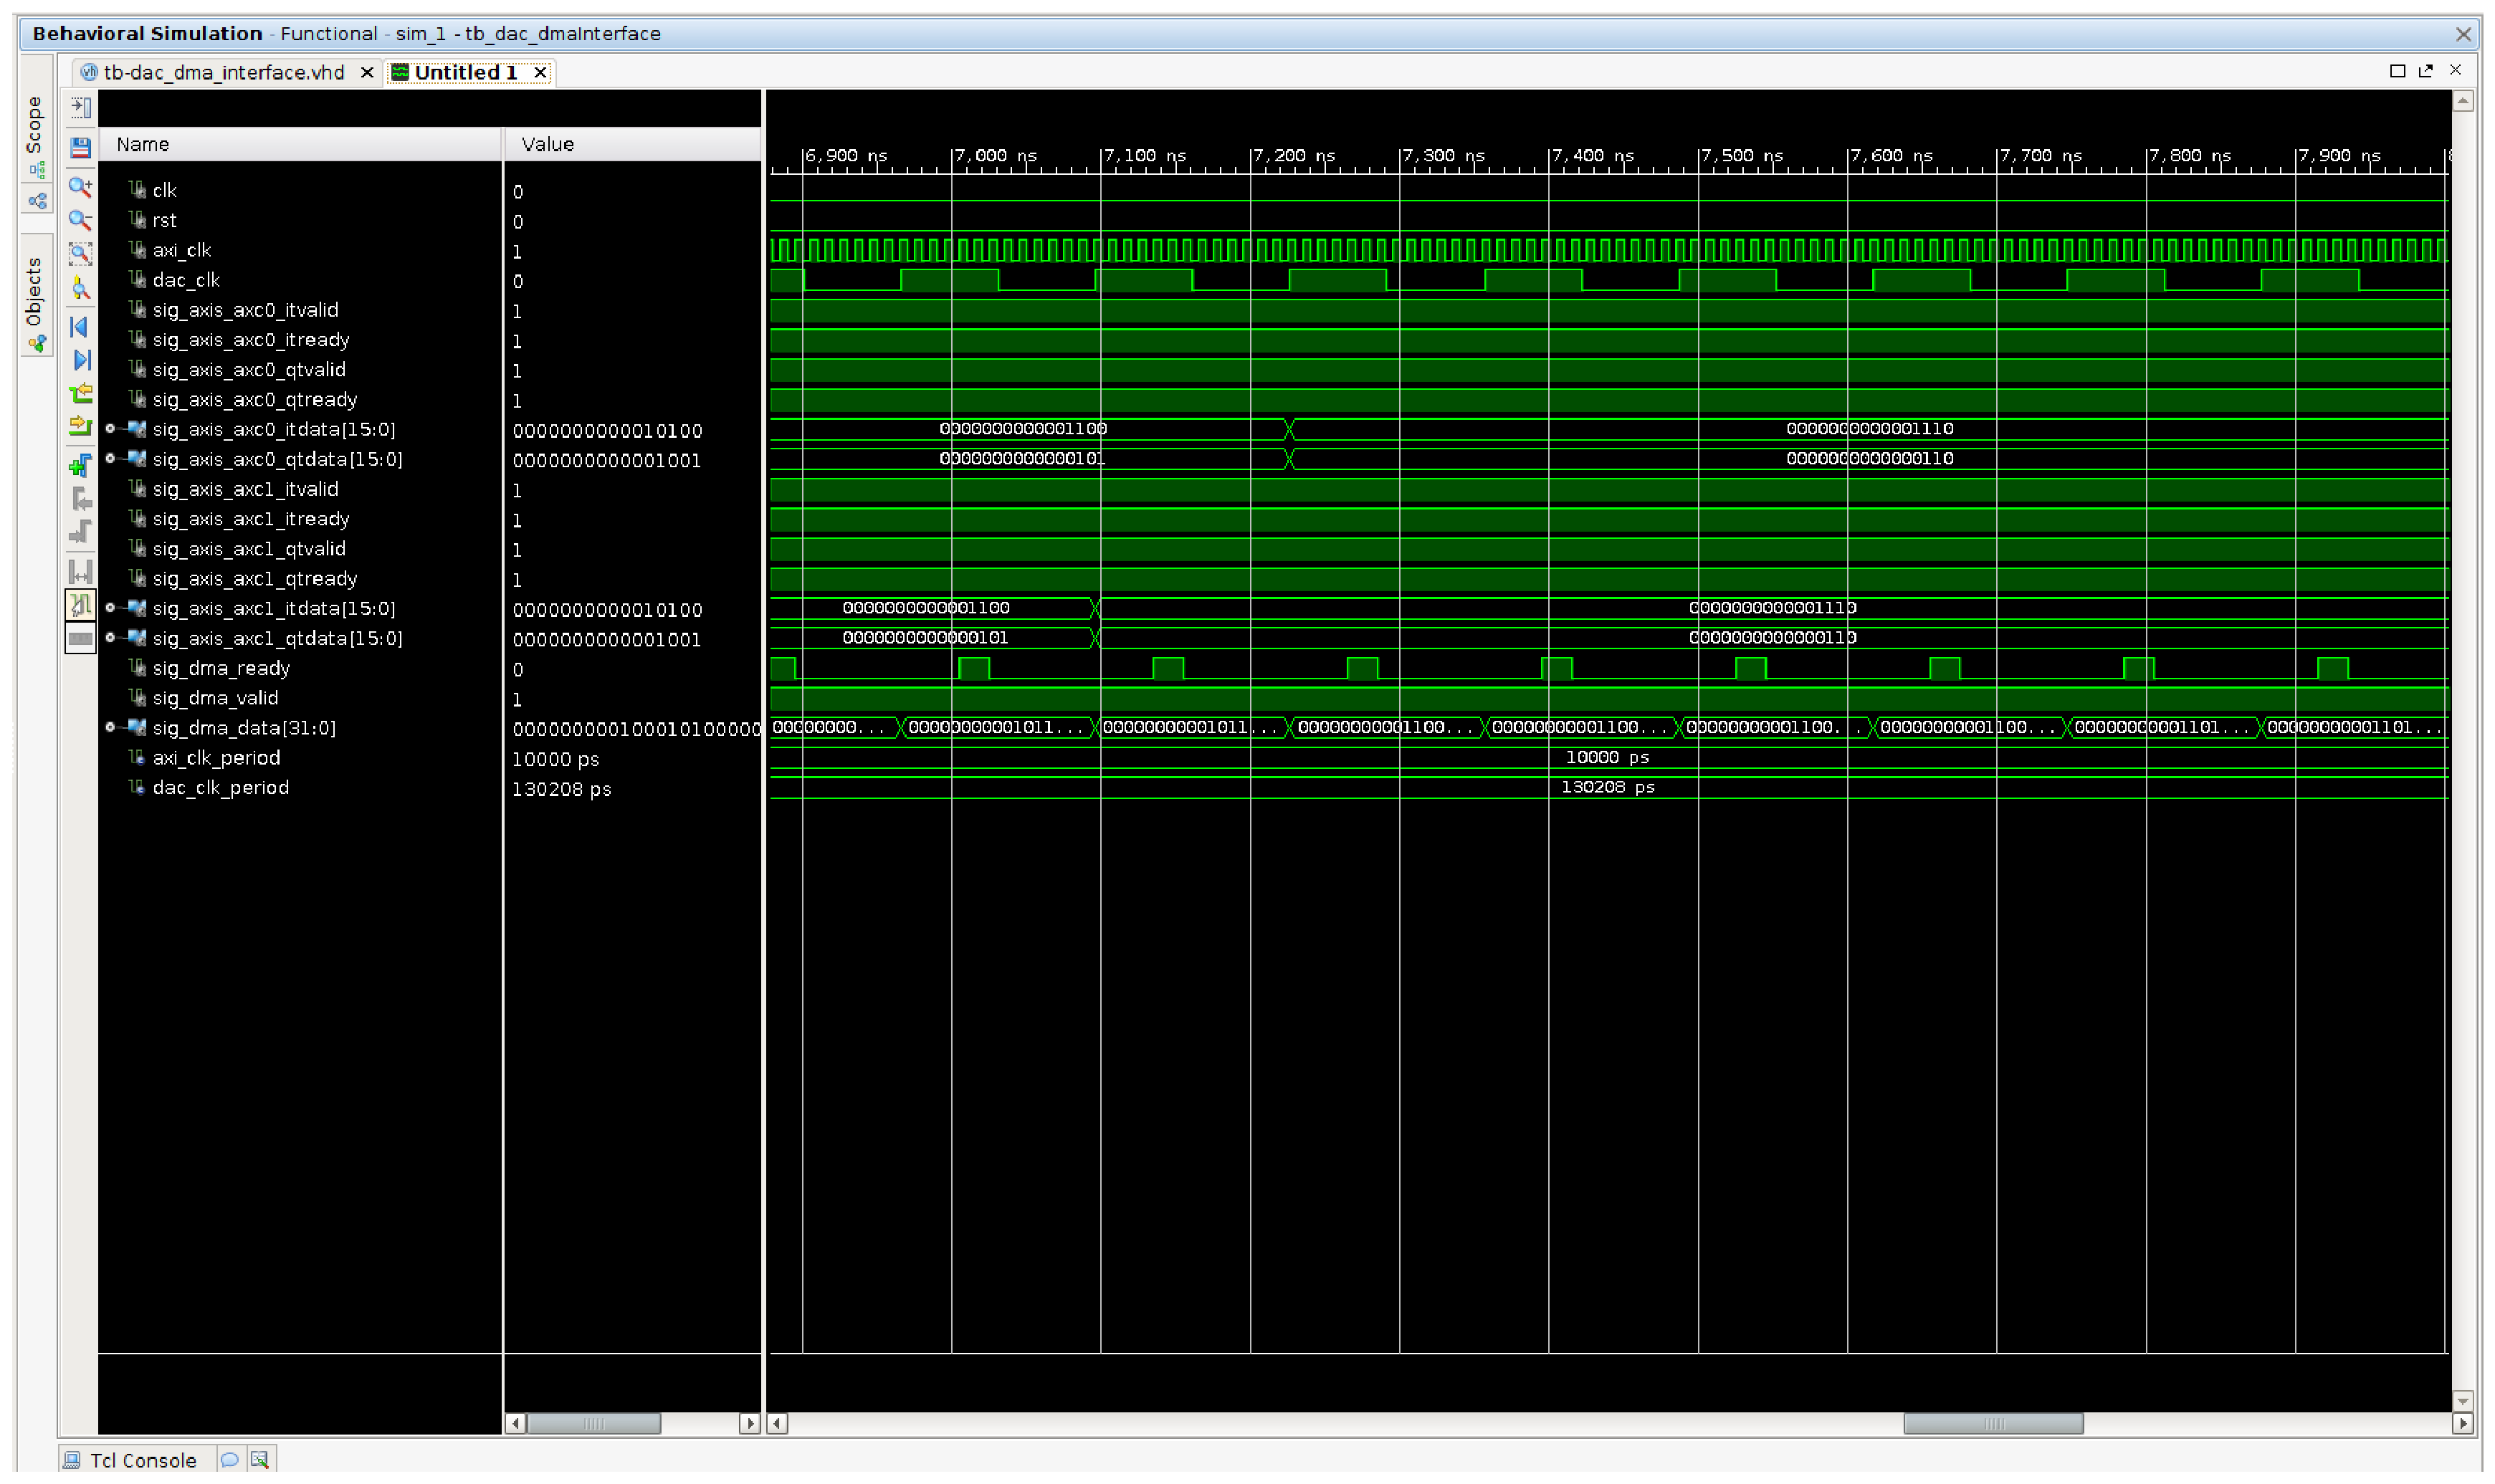
\includegraphics[height=.3\textwidth, width=.85\textwidth,
    trim={{.13\textwidth} {.90\textwidth} {.05\textwidth} {.15\textwidth}},
    clip]{./figures/dac_dmaInterface}
    \caption{ Step 1: DAC-DMA interface block simulation.
    \label{fig:simdacdma}}
\end{figure}

 In Figure \ref{fig:simdac}, the \textit{dacInterface} is simulated and again it
 is possible to obseve the signals \textit{sig\_axis\_axc0\_itdata,
 sig\_axis\_axc0\_qtdata, sig\_axis\_axc1\_itdata and sig\_axis\_axc1\_qtdata}
 being fed to the block and the outputs \textit{sig\_dac\_i0data,
 sig\_dac\_q0data, sig\_dac\_i1data and sig\_dac\_q1data}. The goal in both
 \textit{dac-dmaIterface} and \textit{dacInterface} simulation is to observe
 changes in outputs accompanying \textit{ready and valid} signals of the AXI
 protocol, which are used as a way of controlling the data flow from the
 \textit{DMA}. In such scheme, the \textit{DMA} asserts \textit{valid} whenever
 it can send data. However, it only sends the data when fed by a ready signal,
 meaning that the reading block can read the \textit{DMA} data.

\begin{figure}[htbp]
    \centering
    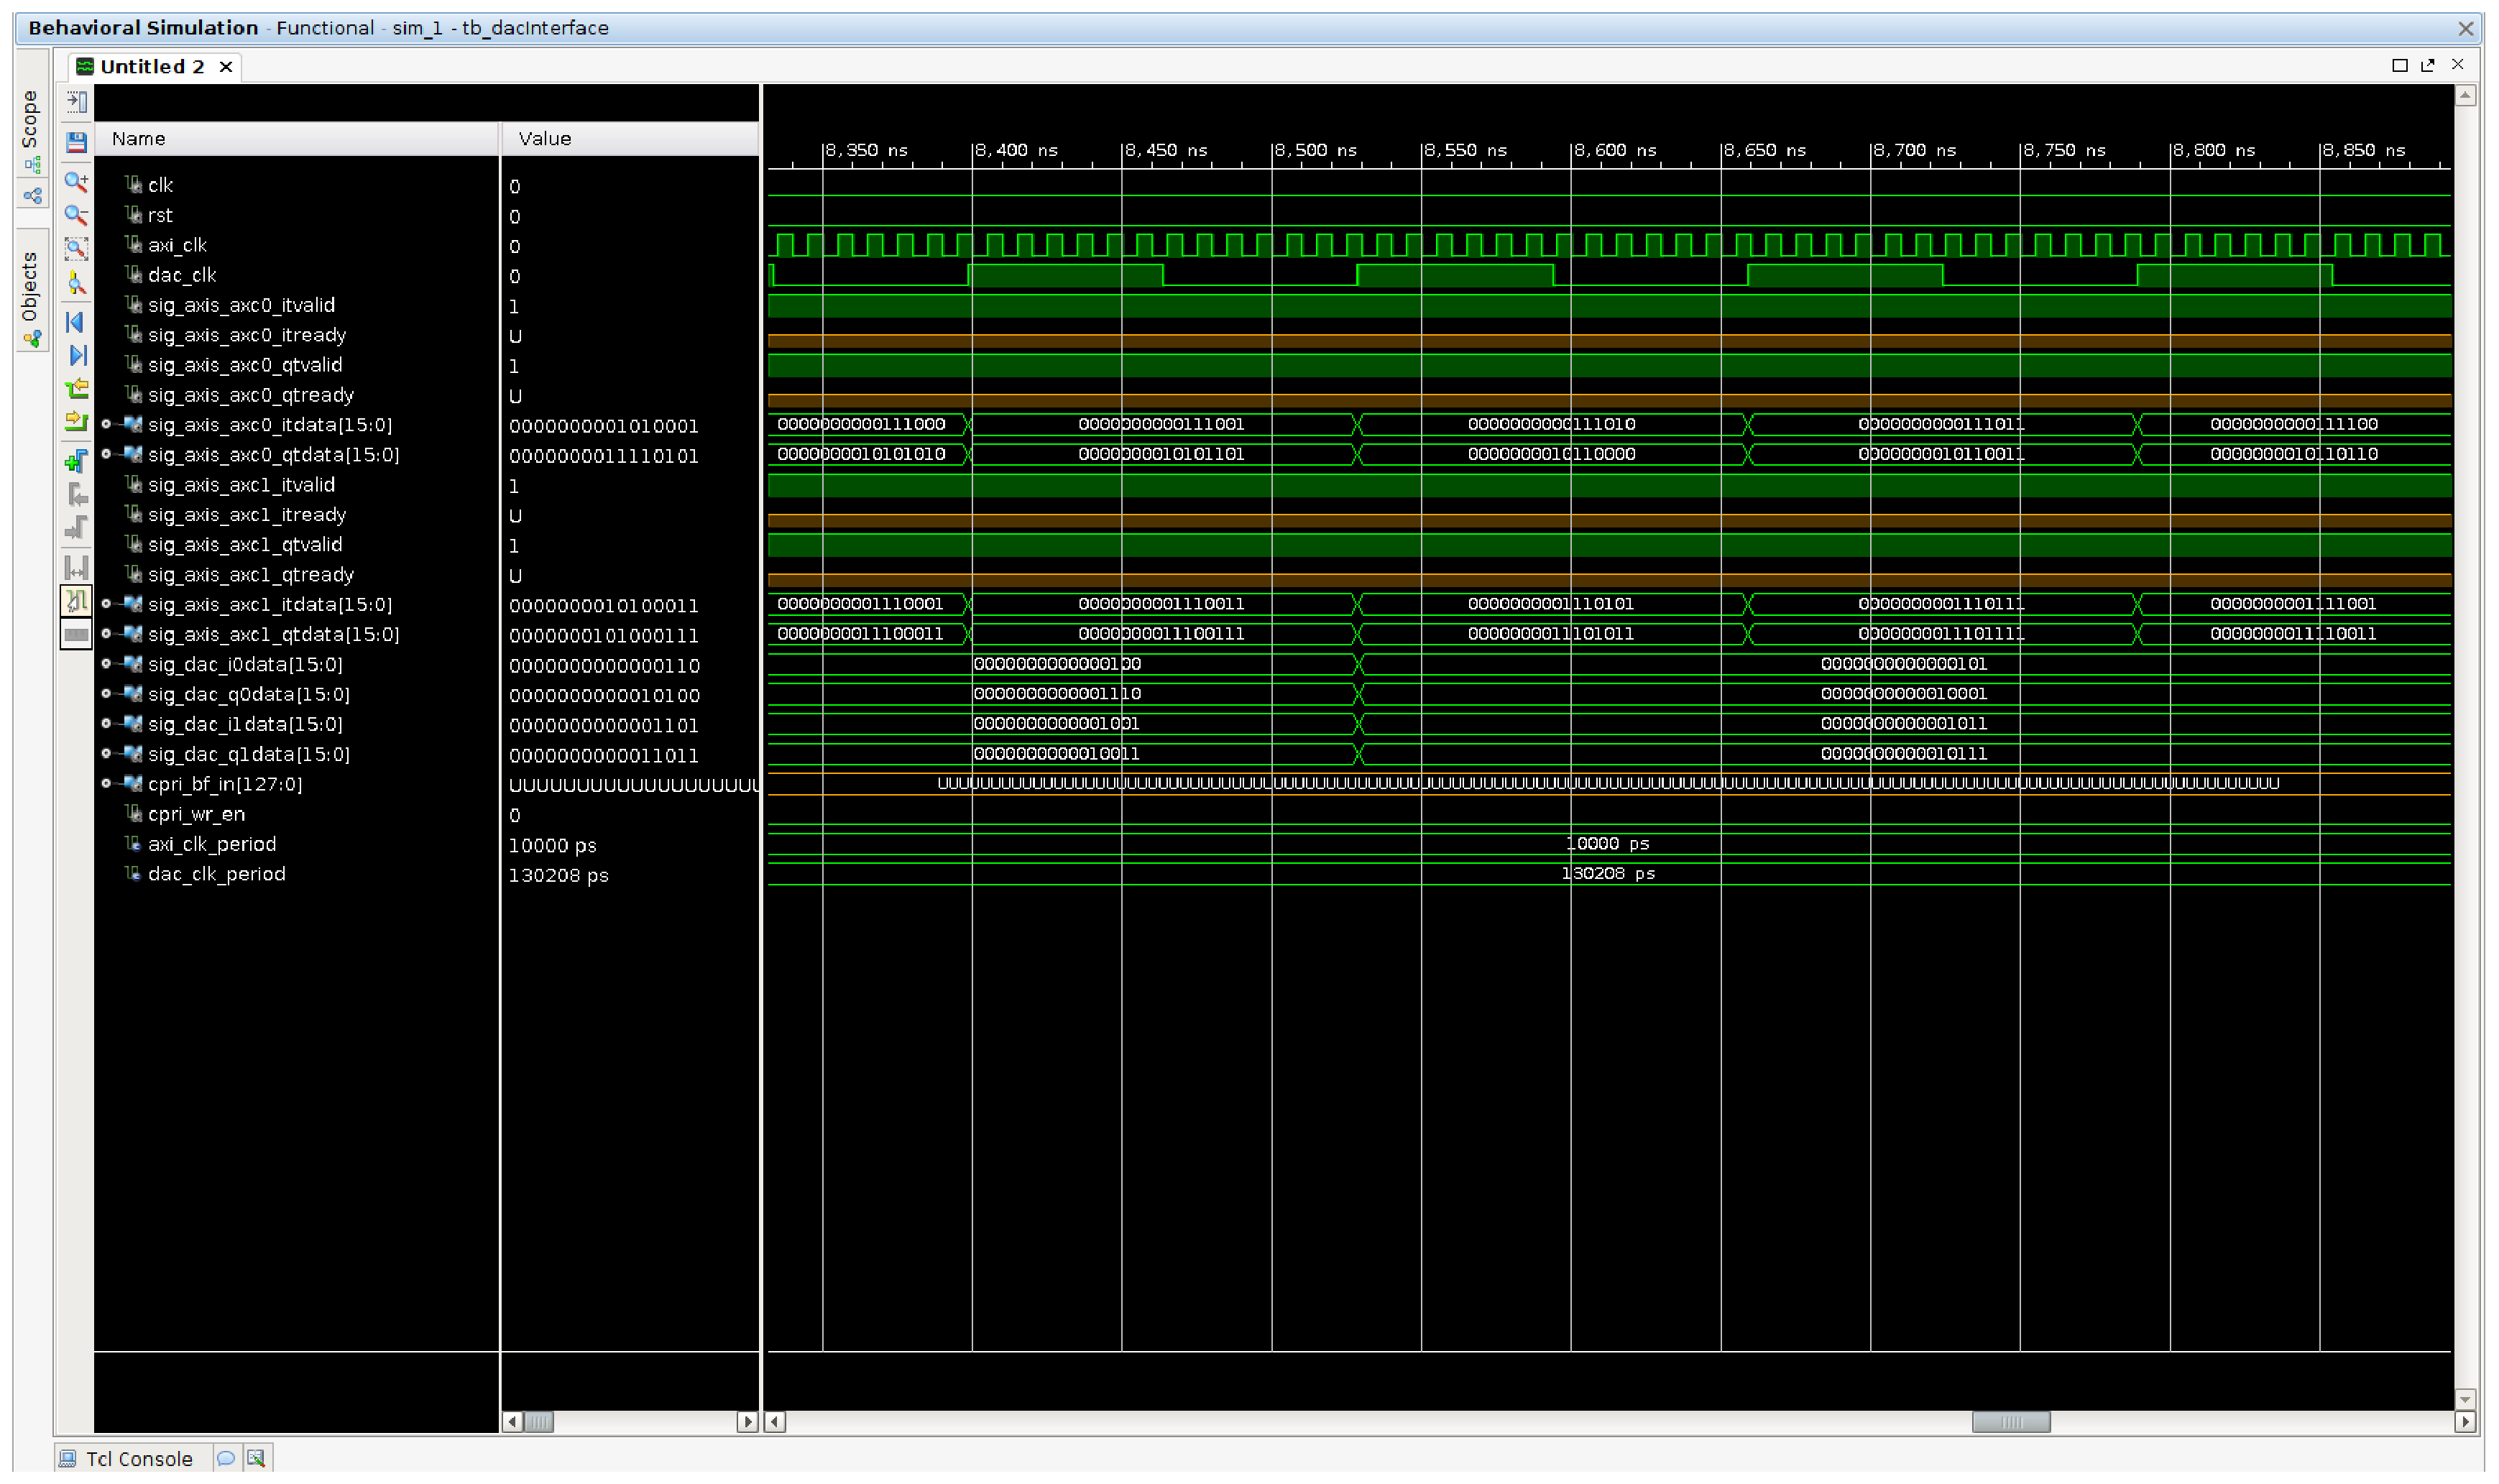
\includegraphics[height=.4\textwidth, width=1\textwidth,
    trim={{.13\textwidth} {.8\textwidth} {.05\textwidth} {.15\textwidth}},
    clip]{./figures/dacInterface}
    \caption{ Step 2: DAC interface block simulation.
    \label{fig:simdac}}
\end{figure}

In the final simulation of the transmitting interface the whole transmit chain
blocks were simulated together, which allows the evaluation of the behavior of
the whole transmit interface block. In Figure \ref{fig:simtxif} it is possible
to watch the \textit{DMA} data in the signal in \textit{dac-dmaIterface} and the
outputs which would feed the \textit{AD9361} two \textit{DACs} in the signals
\textit{sig\_dac\_i0data, sig\_dac\_q0data, sig\_dac\_i1data and
sig\_dac\_q1data}. Again, it is possible to note the data changes when the
\textit{ready and valid} changes. Another interesting thing to observe is the
two clock variables \textit{axi\_clk} and \textit{dac\_clk} which represent both
AXI system clock $ 100 MHz$ and the DAC clock $40 MHz$, this difference
justifies the use of such interface.


\begin{figure}[htbp]
    \centering
    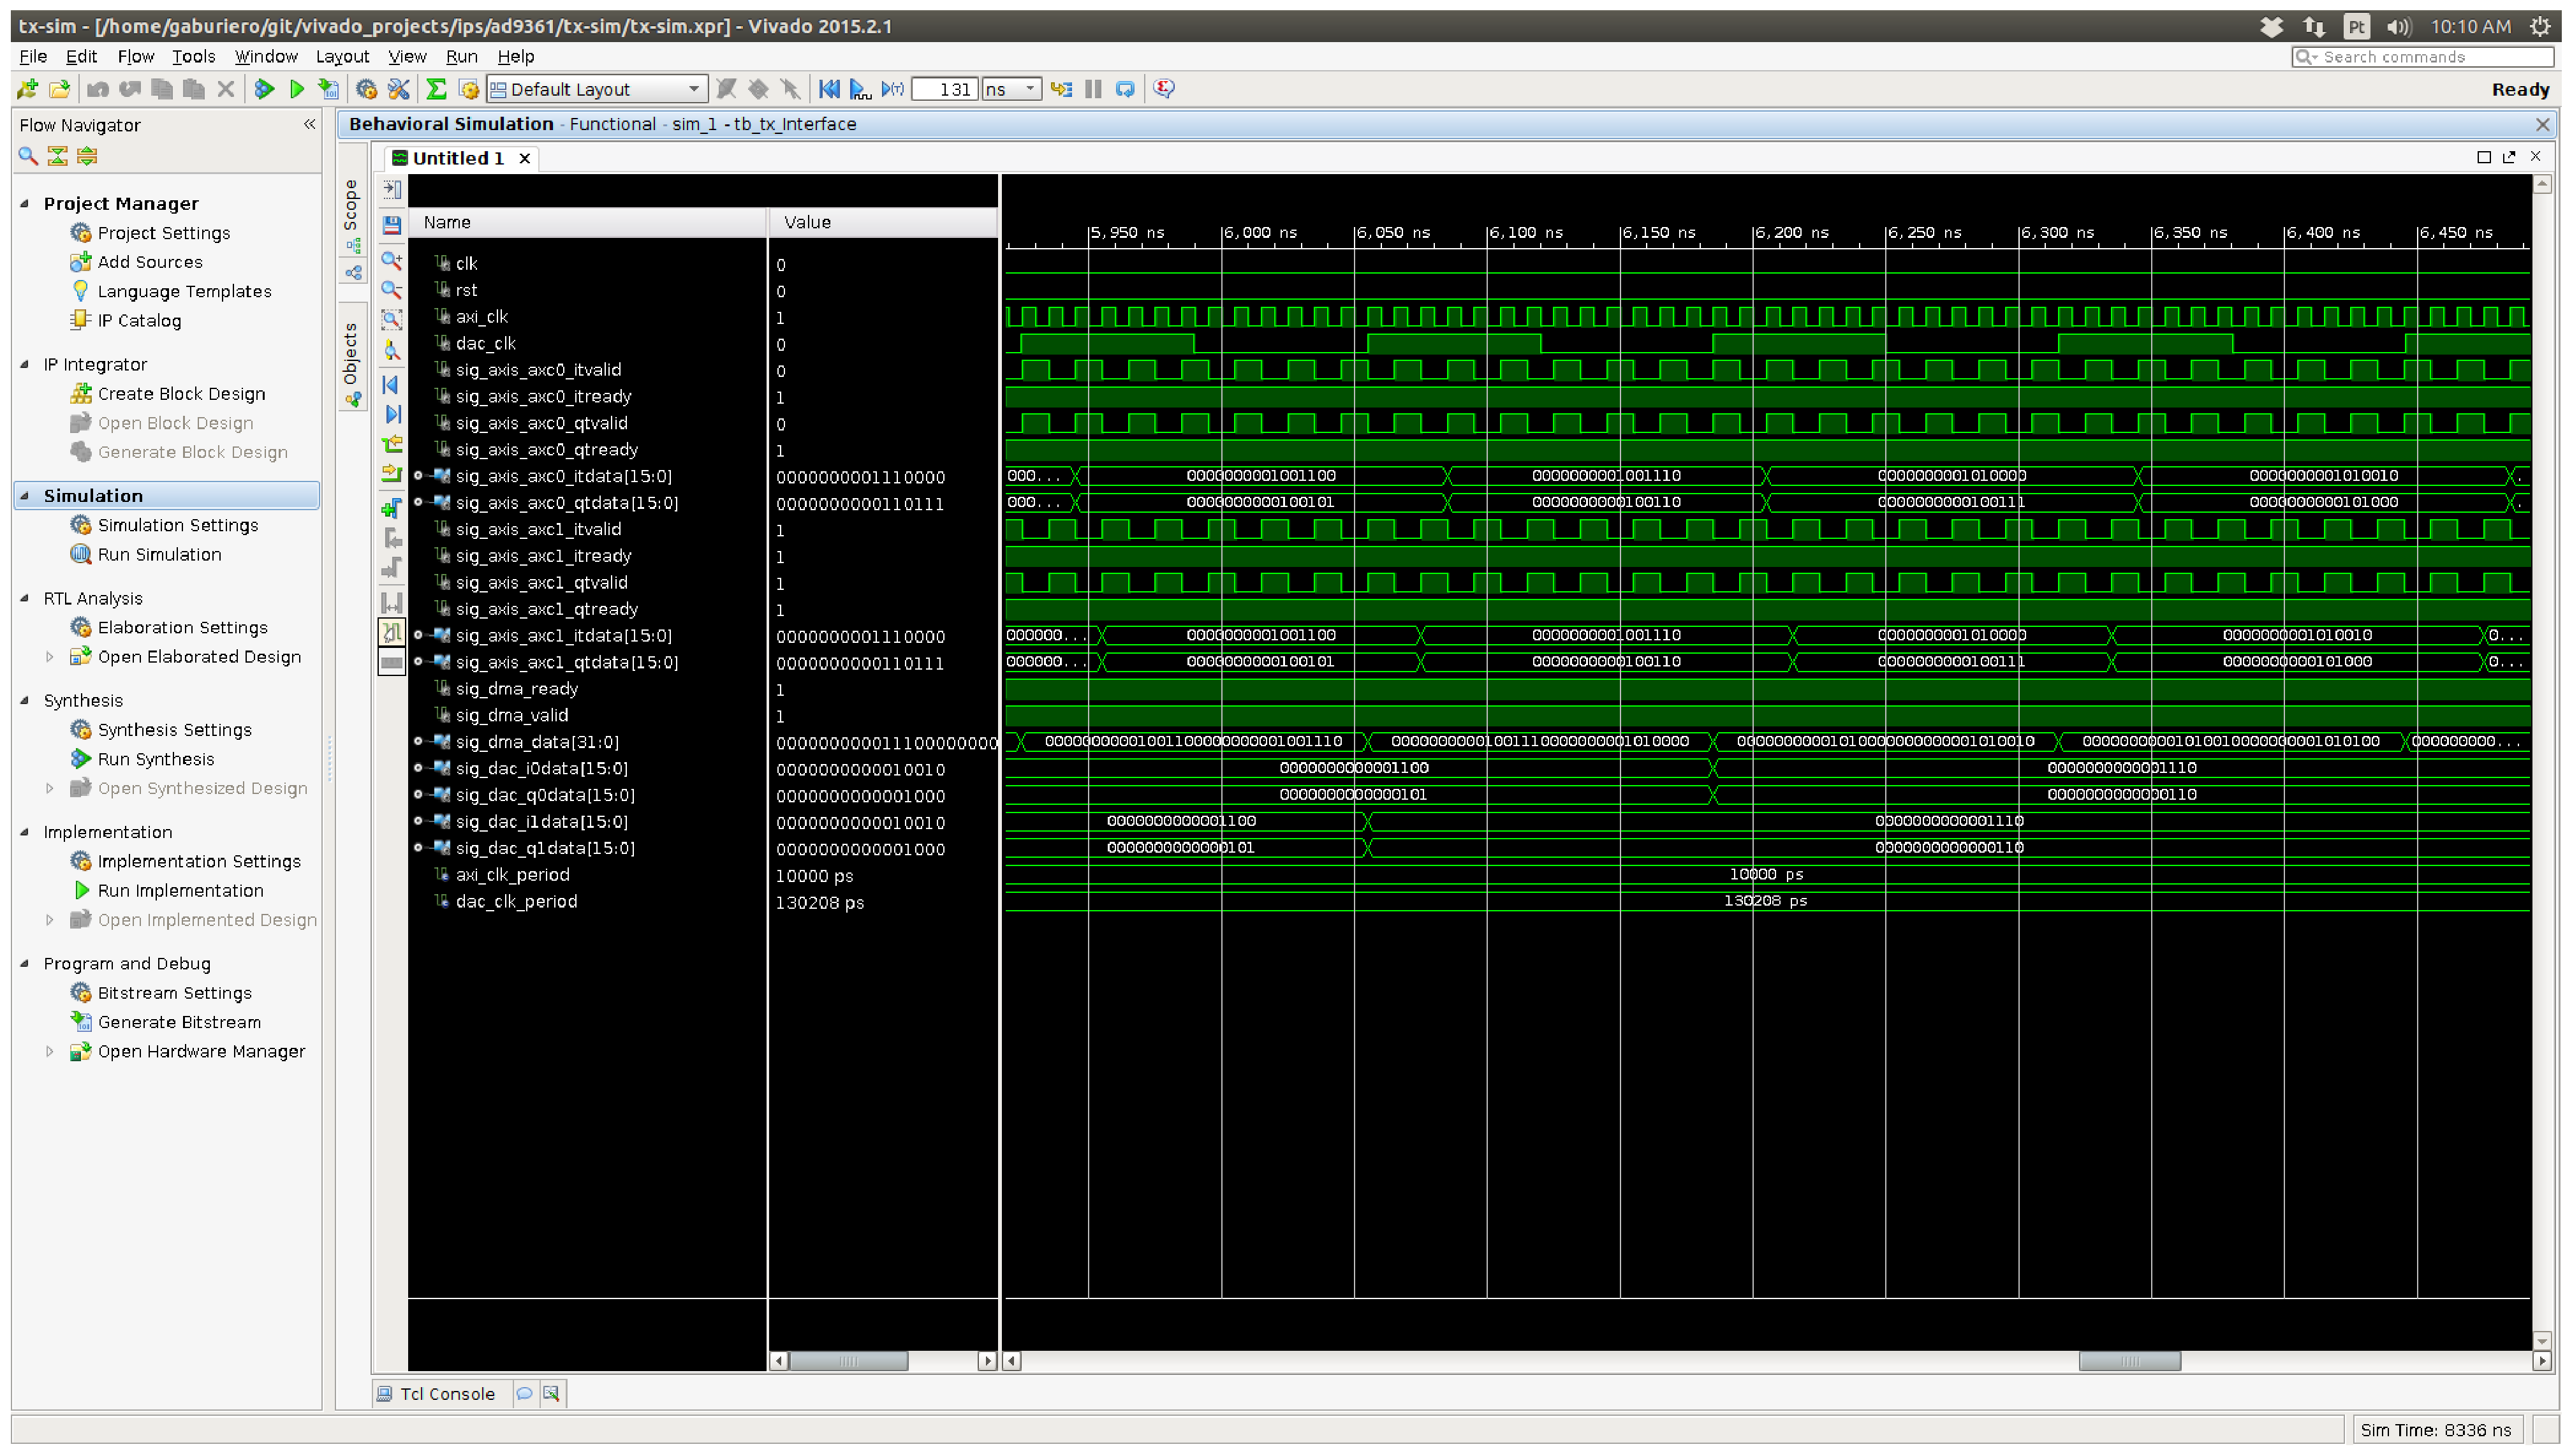
\includegraphics[width=1\textwidth,
    trim={{.67\textwidth} {.7\textwidth} {.05\textwidth} {.3\textwidth}},
    clip]{./figures/txInterface}
    \caption{ Step 3: transmitting interface block simulation.
    \label{fig:simtxif}}
\end{figure}

\subsection{Receive (ADC) Interface Simulation}

As stated before in Section \ref{impl:setup}, the DAC interface is simple
because the data input is already limited by the DAC clock, so there is no need
to make any structure to control the data flow like in the DAC interface.

In Figure \ref{fig:simdac} it is possible to see the output and wave diagram in
the simulation window. Since the \textit{adcInterface} is much simpler, because
the data input is already limited by the \textit{AD9361} clock as explained in
Section \ref{impl:setup}. The signals \textit{sig\_rx\_i0\_data,
sig\_rx\_q0\_data, sig\_rx\_i1\_data, sig\_rx\_q1\_data} represent the outputs
from both \textit{DACs} and \textit{dout} is the data that will be fed to the
\textit{DMA}. In Figure \ref{fig:simdac} it is possible to observe that the 16
bit input data streams \textit{sig\_rx\_i0\_data, sig\_rx\_q0\_data,
sig\_rx\_i1\_data, sig\_rx\_q1\_data} are being concatenated into 32 bits
\textit{dout [31:0]}and are being fed to the DMA block in the output and the
channels are being alternated in the DMA input.

\begin{figure}[htbp]
    \centering
    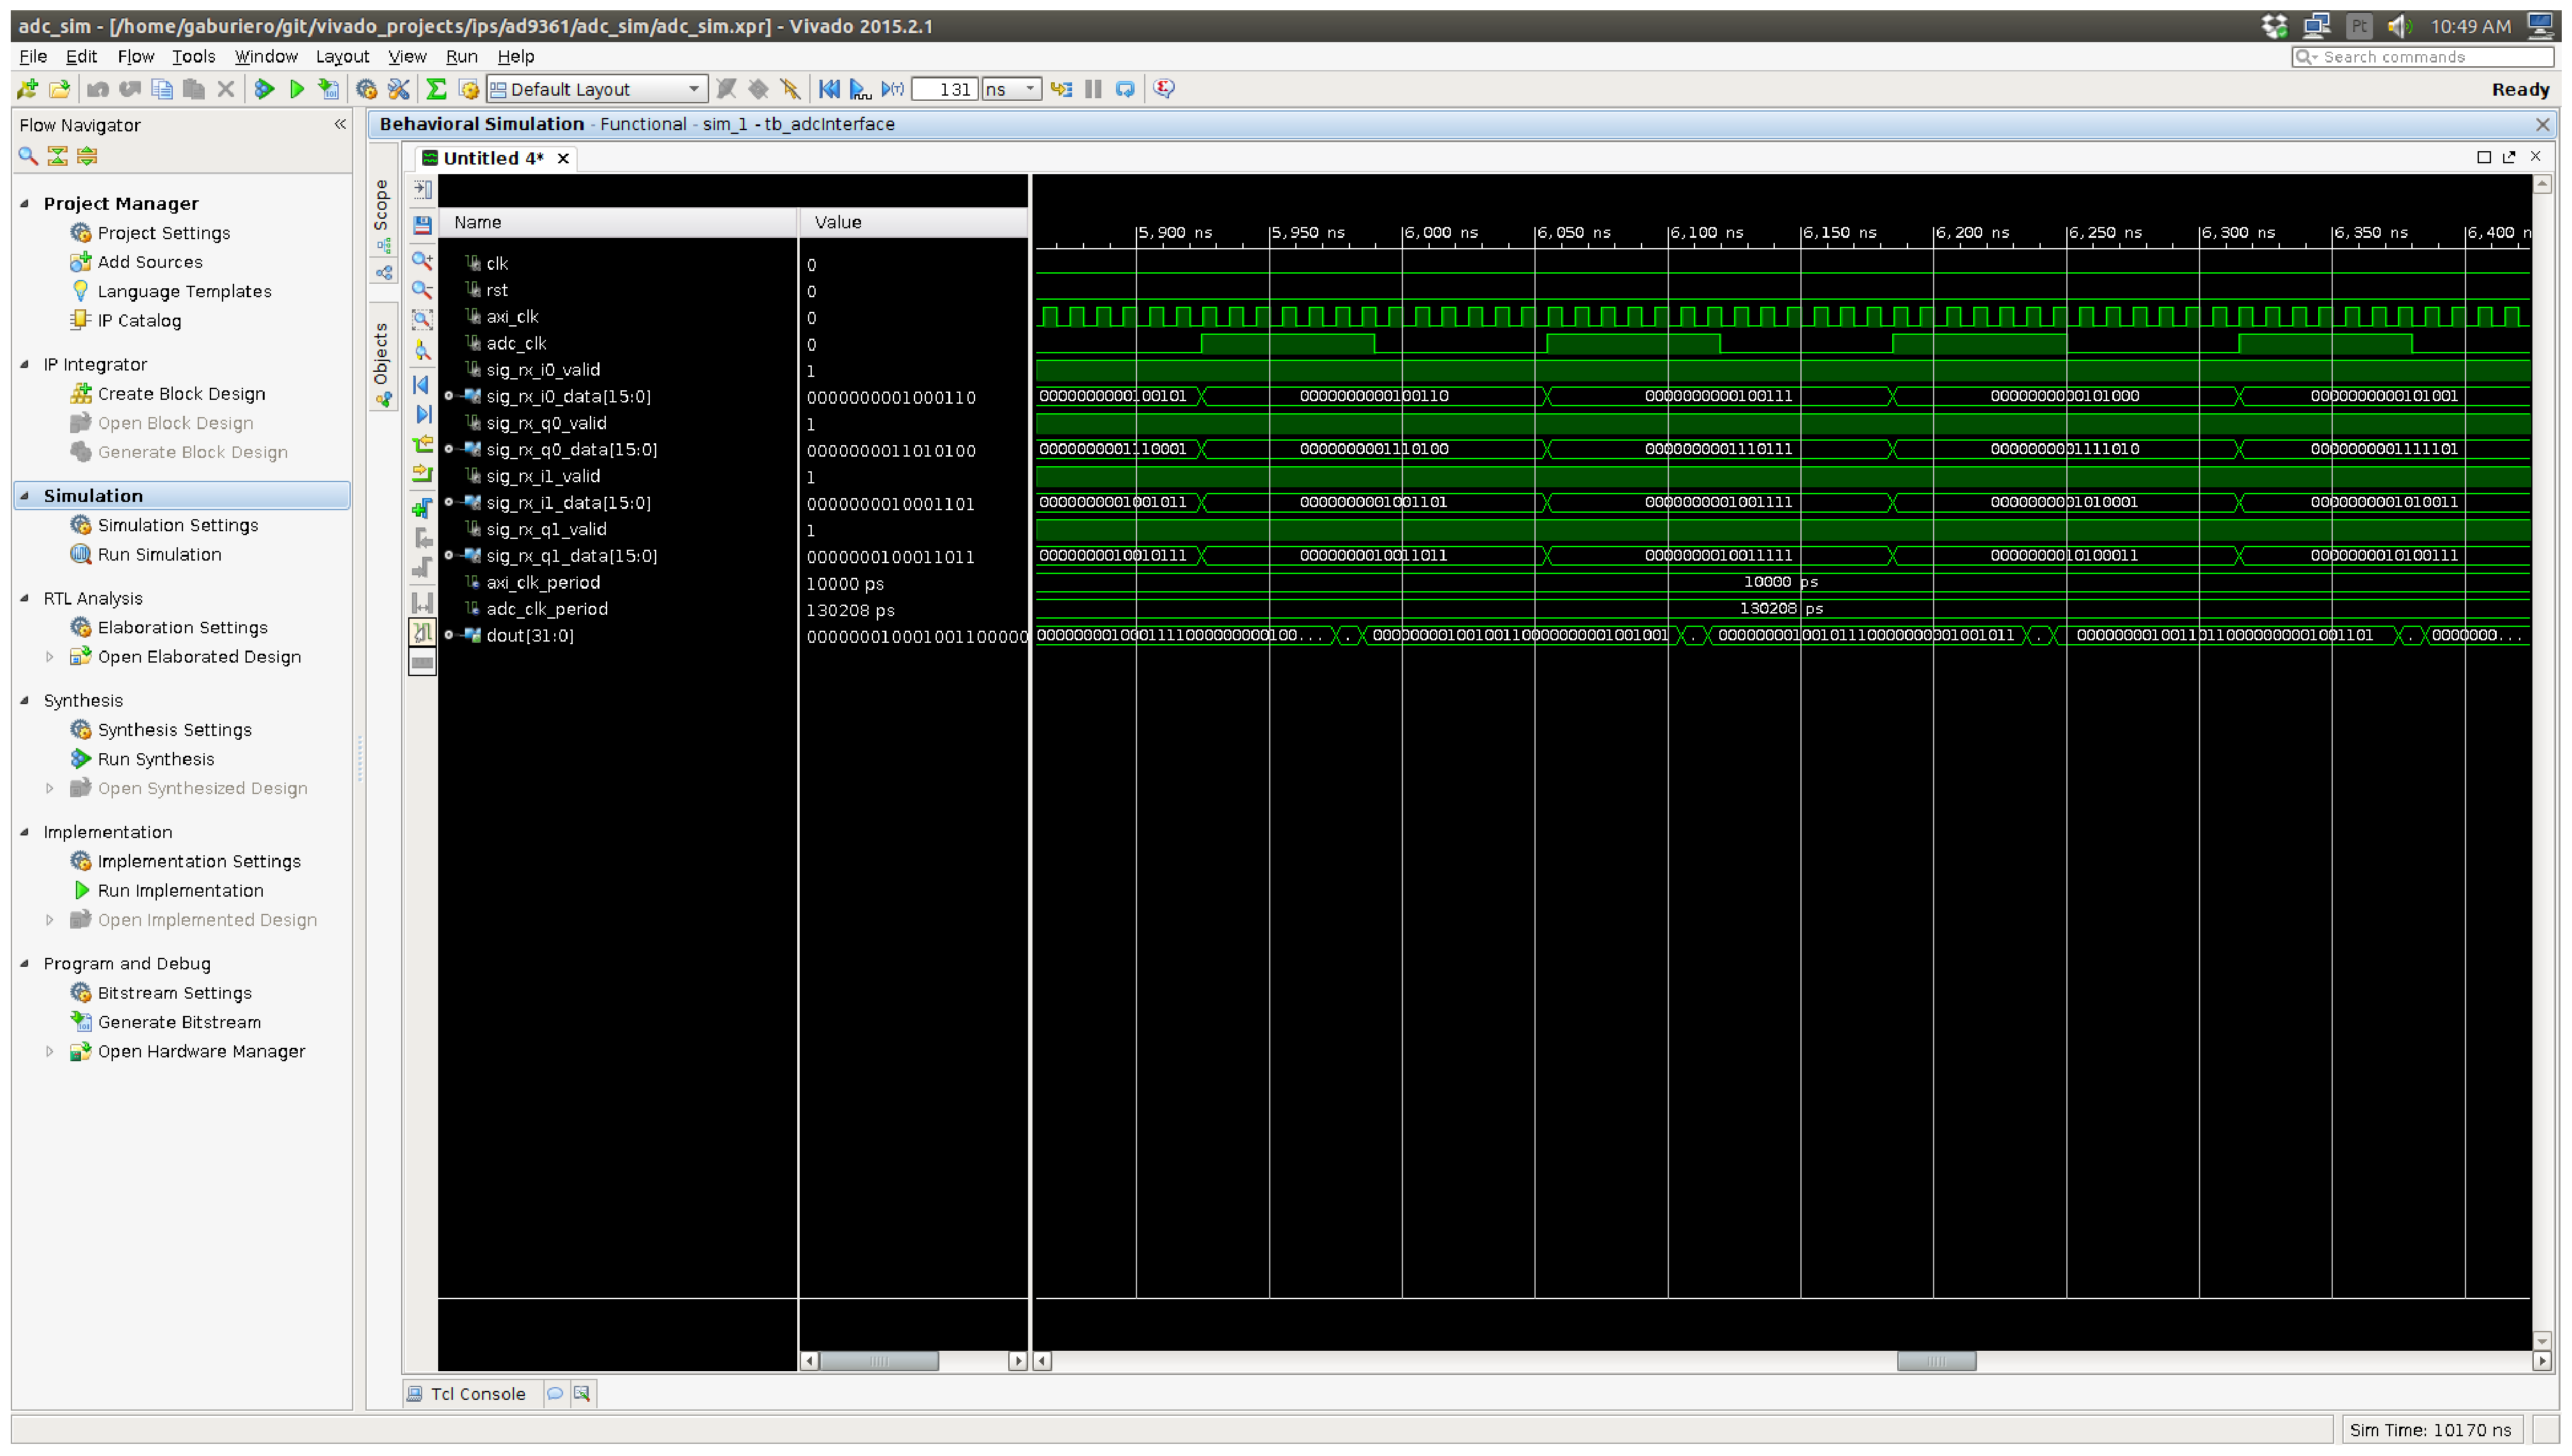
\includegraphics[width=0.95\textwidth,
    trim={{.13\textwidth} {.95\textwidth} {.05\textwidth} {.15\textwidth}},
    clip]{./figures/adcInterface}
    \caption{ ADC interface block simulation.
    \label{fig:simadc}}
\end{figure}



\section{Transmission Tests (Downlink)}
\label{result:dac}

The transmission tests aim to evaluate a downlink LTE transmission, namely a
transmission from the eNodeB to the UE. In this transmission, an LTE waveform
generated offline in MATLAB was loaded into the FPGA memory by putting them in a
header file. The DMA engine was, then, configured to read from the memory region
were the waveform was loaded and the samples were sent read them and the DAC
shall make an analog output. Figure 5.14 presents the DAC control signals sent
to the data interface block in order to control the data flow. It makes a
back-pressure in the DMA engine controlling if DMA reads or not data from
memory. The DMA Engine reading output can be seen in Figures
\ref{fig:dataflowdig} and \ref{fig:dataflowana}, digital and analog waveforms
respectively.

It is possible to configure in the driver if the AD9361 outputs or not a clock
in a special clock\_output pin, so in order to evaluate frequency and clock
quality, Figure \ref{fig:dacclk} shows the clock output from the AD9361. Figure
\ref{fig:lte5m} show the output spectrum of the LTE analog wave outputted from
the FMComms2 board.

In Figure \ref{fig:evm} it is possible to observe the EVM measurements of this
setup output waveform, in the bottom of the figure there is the spectrum in the
left and the constellation in the right.

\begin{figure}[htbp]
    \centering
    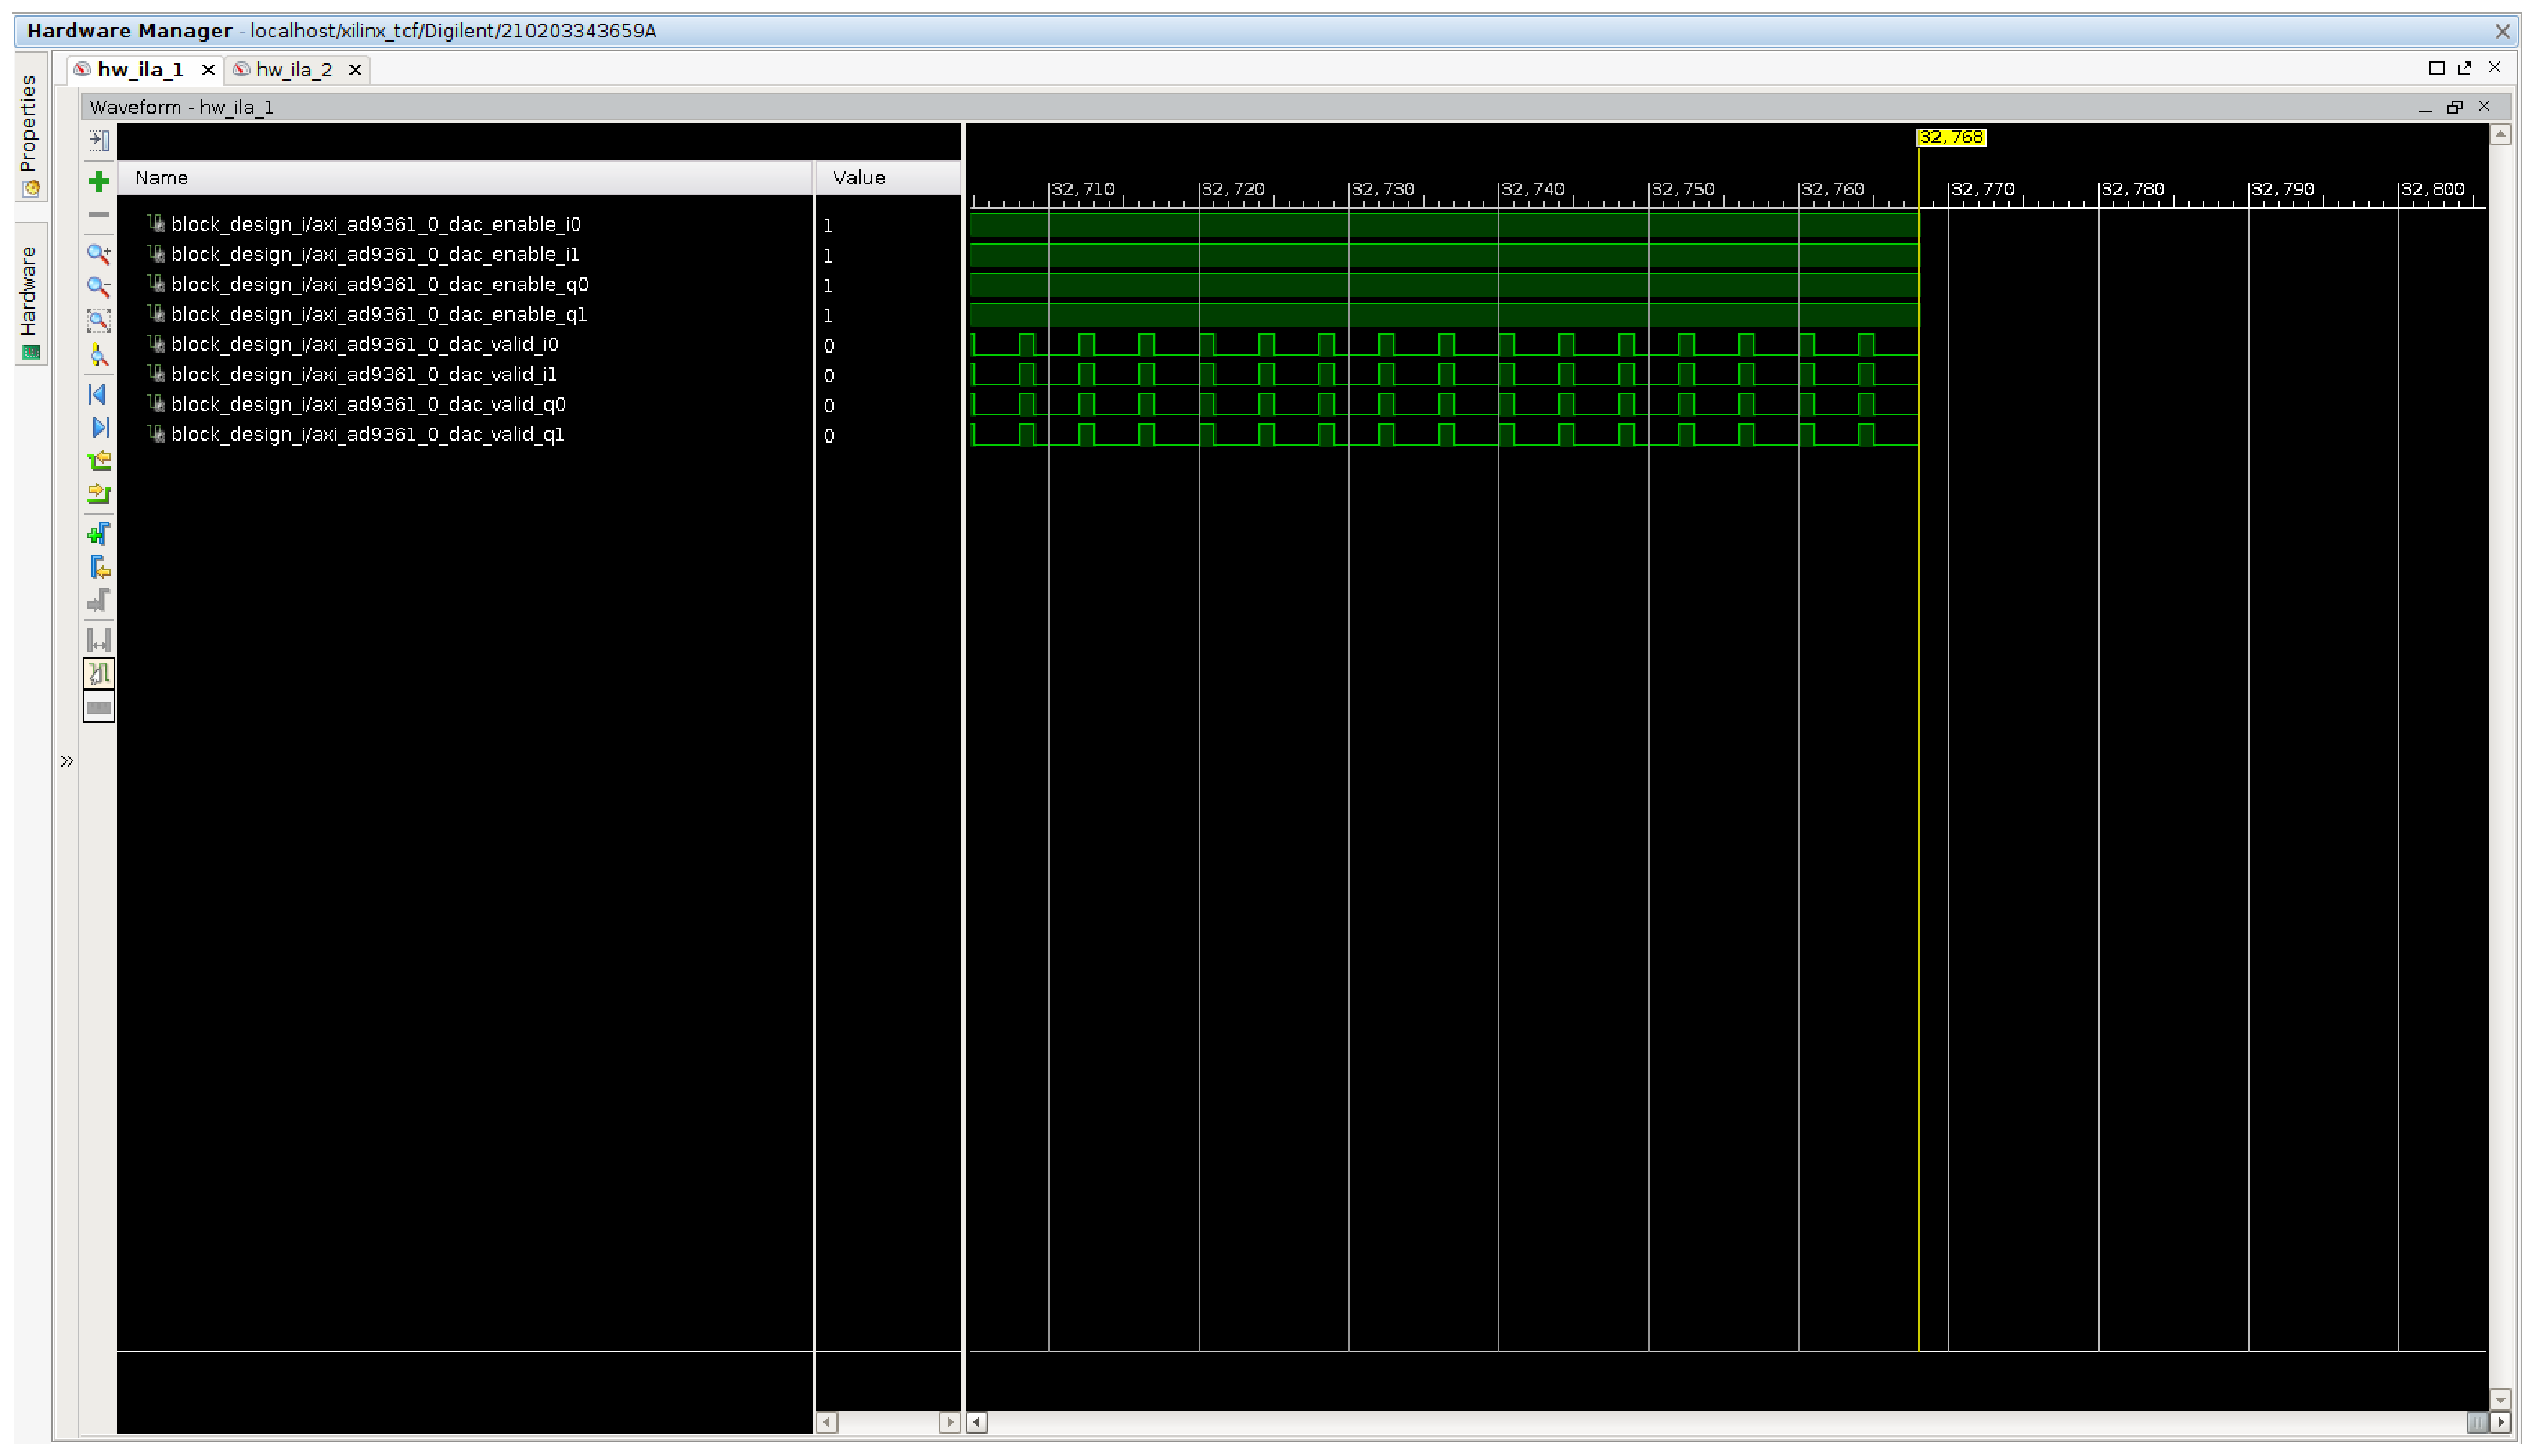
\includegraphics[width=1\textwidth,
    trim={{.15\textwidth} {1.2\textwidth} {.7\textwidth} {.16\textwidth}},
    clip]{./figures/dac_signals}
    \caption{ DAC signals controlling data reading.
    \label{fig:dacsignals}}
\end{figure}

\begin{figure}[htbp]
    \centering
    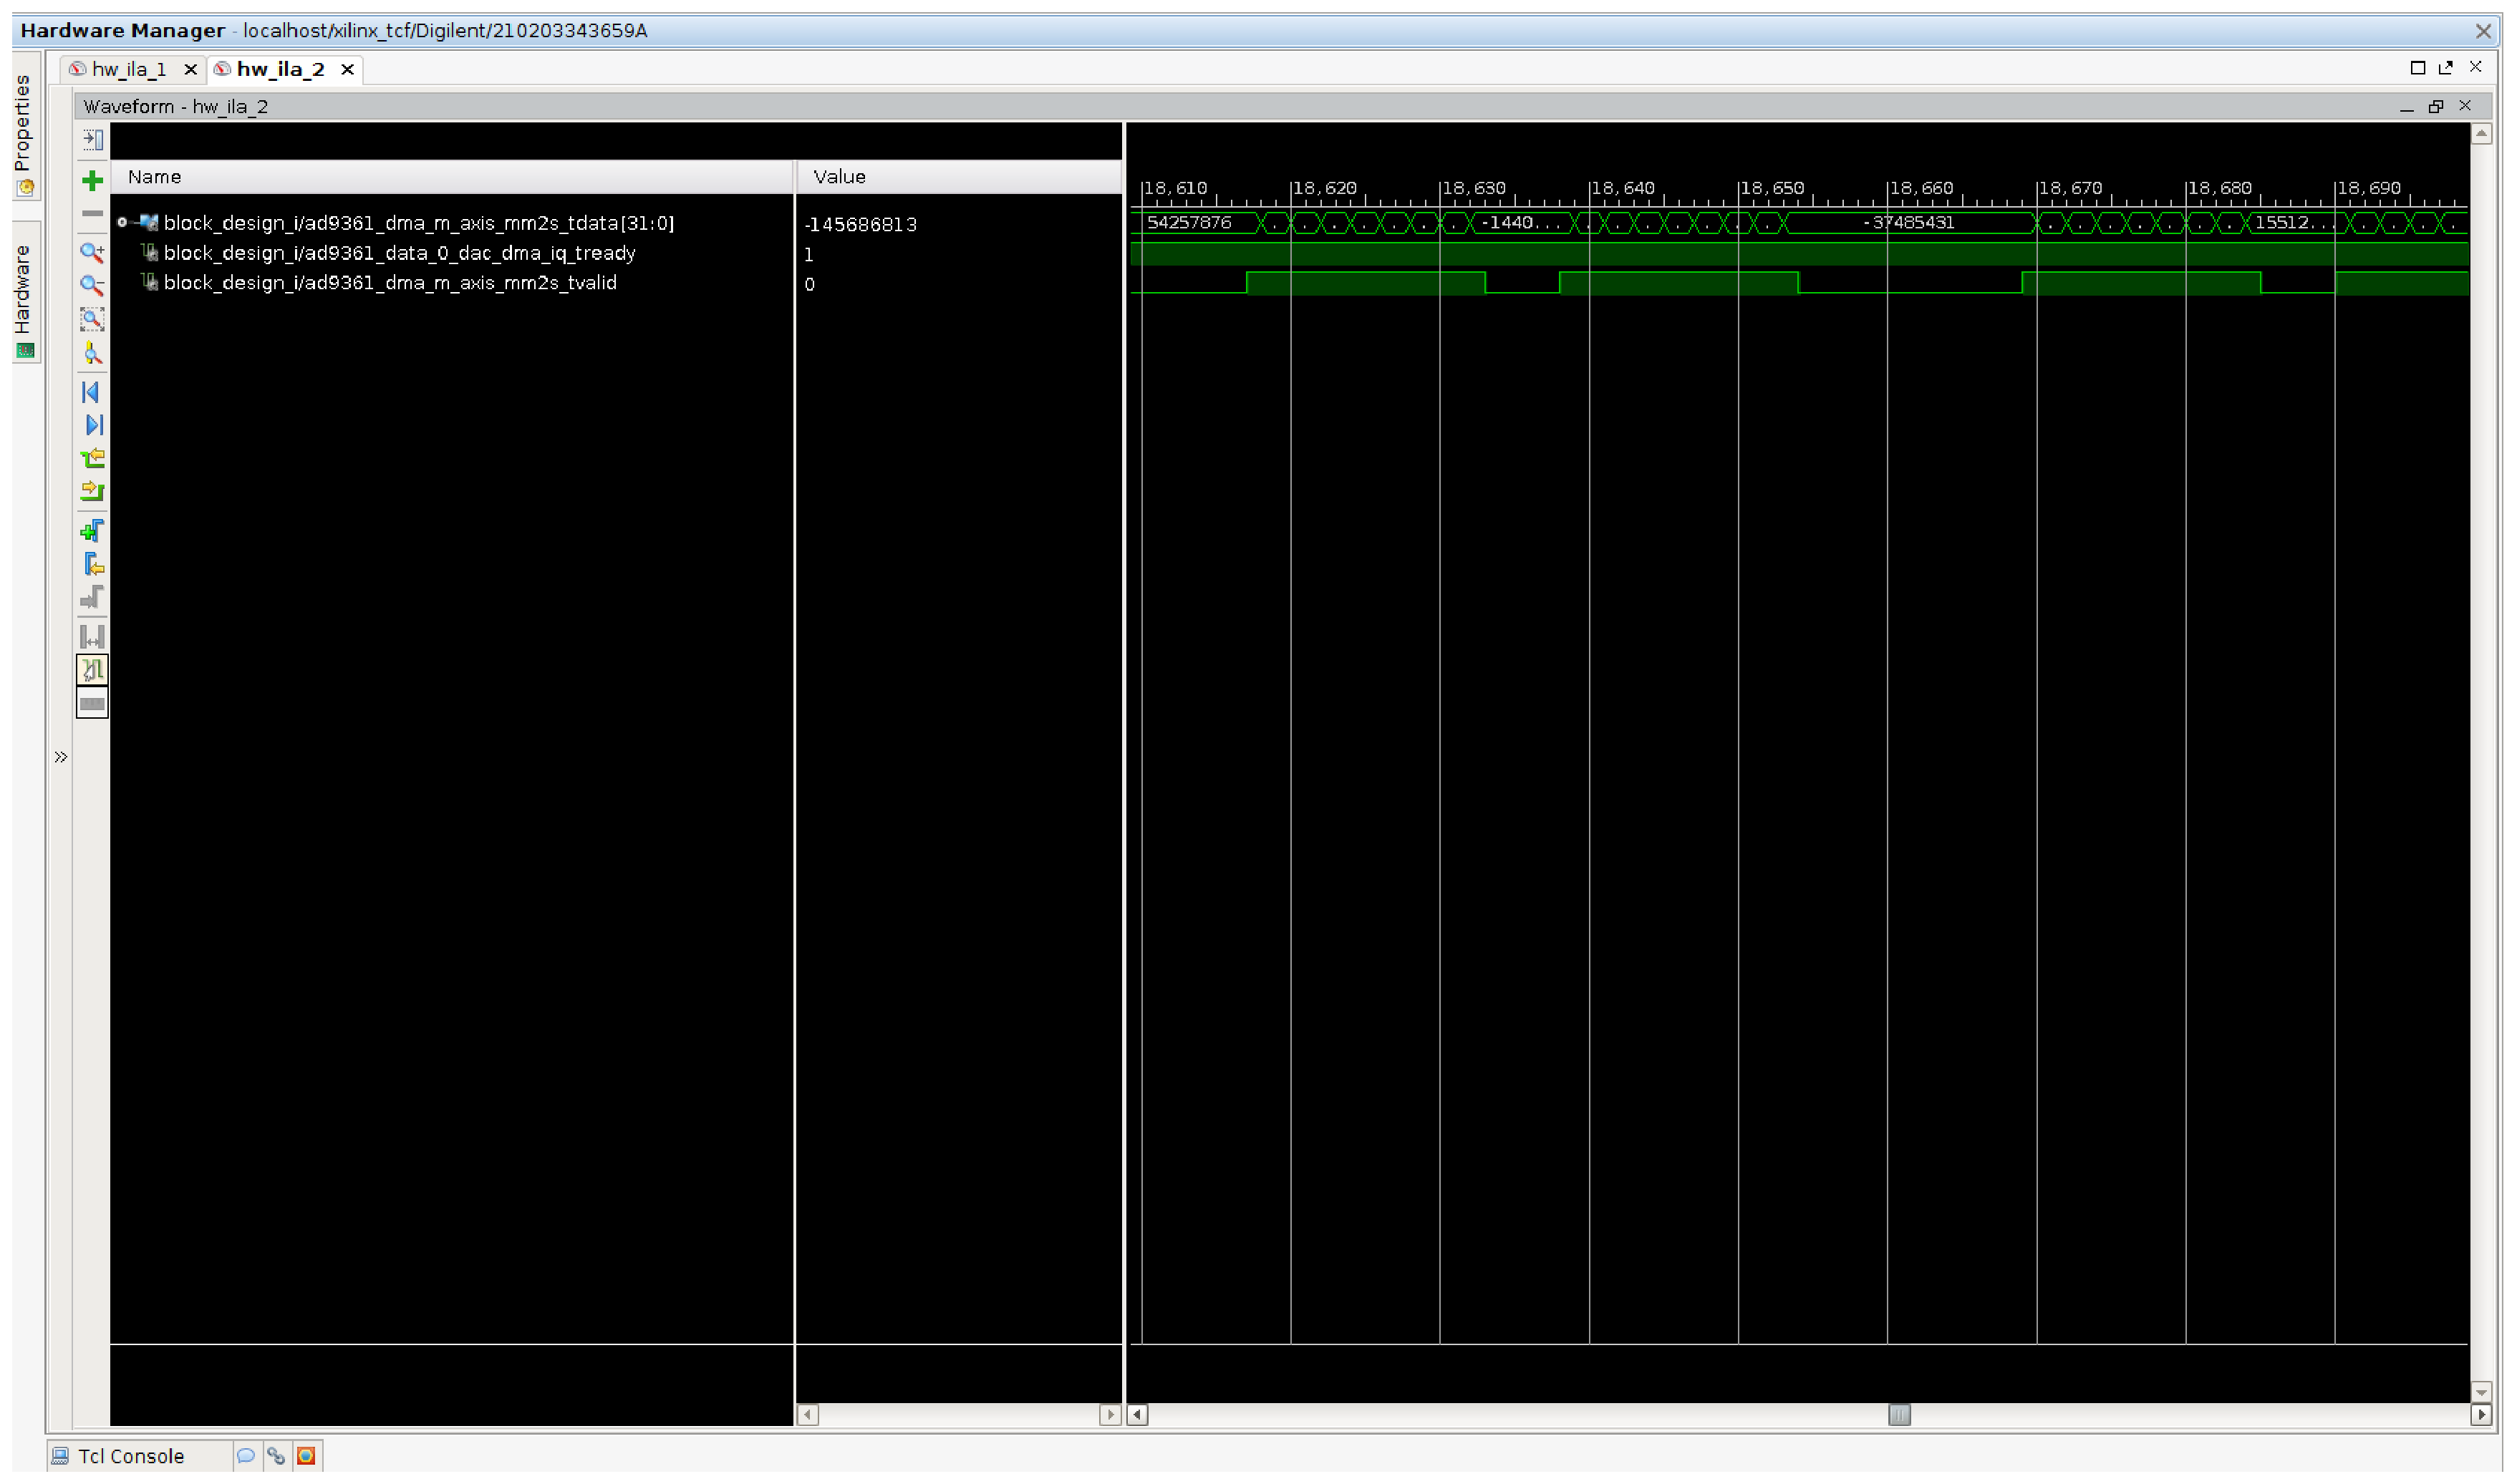
\includegraphics[width=1\textwidth,
    trim={{.15\textwidth} {1.3\textwidth} {.05\textwidth} {.16\textwidth}},
    clip]{./figures/ila_dataflow}
    \caption{ Digital data read from memory by DMA.
    \label{fig:dataflowdig}}
\end{figure}

\begin{figure}[htbp]
    \centering
    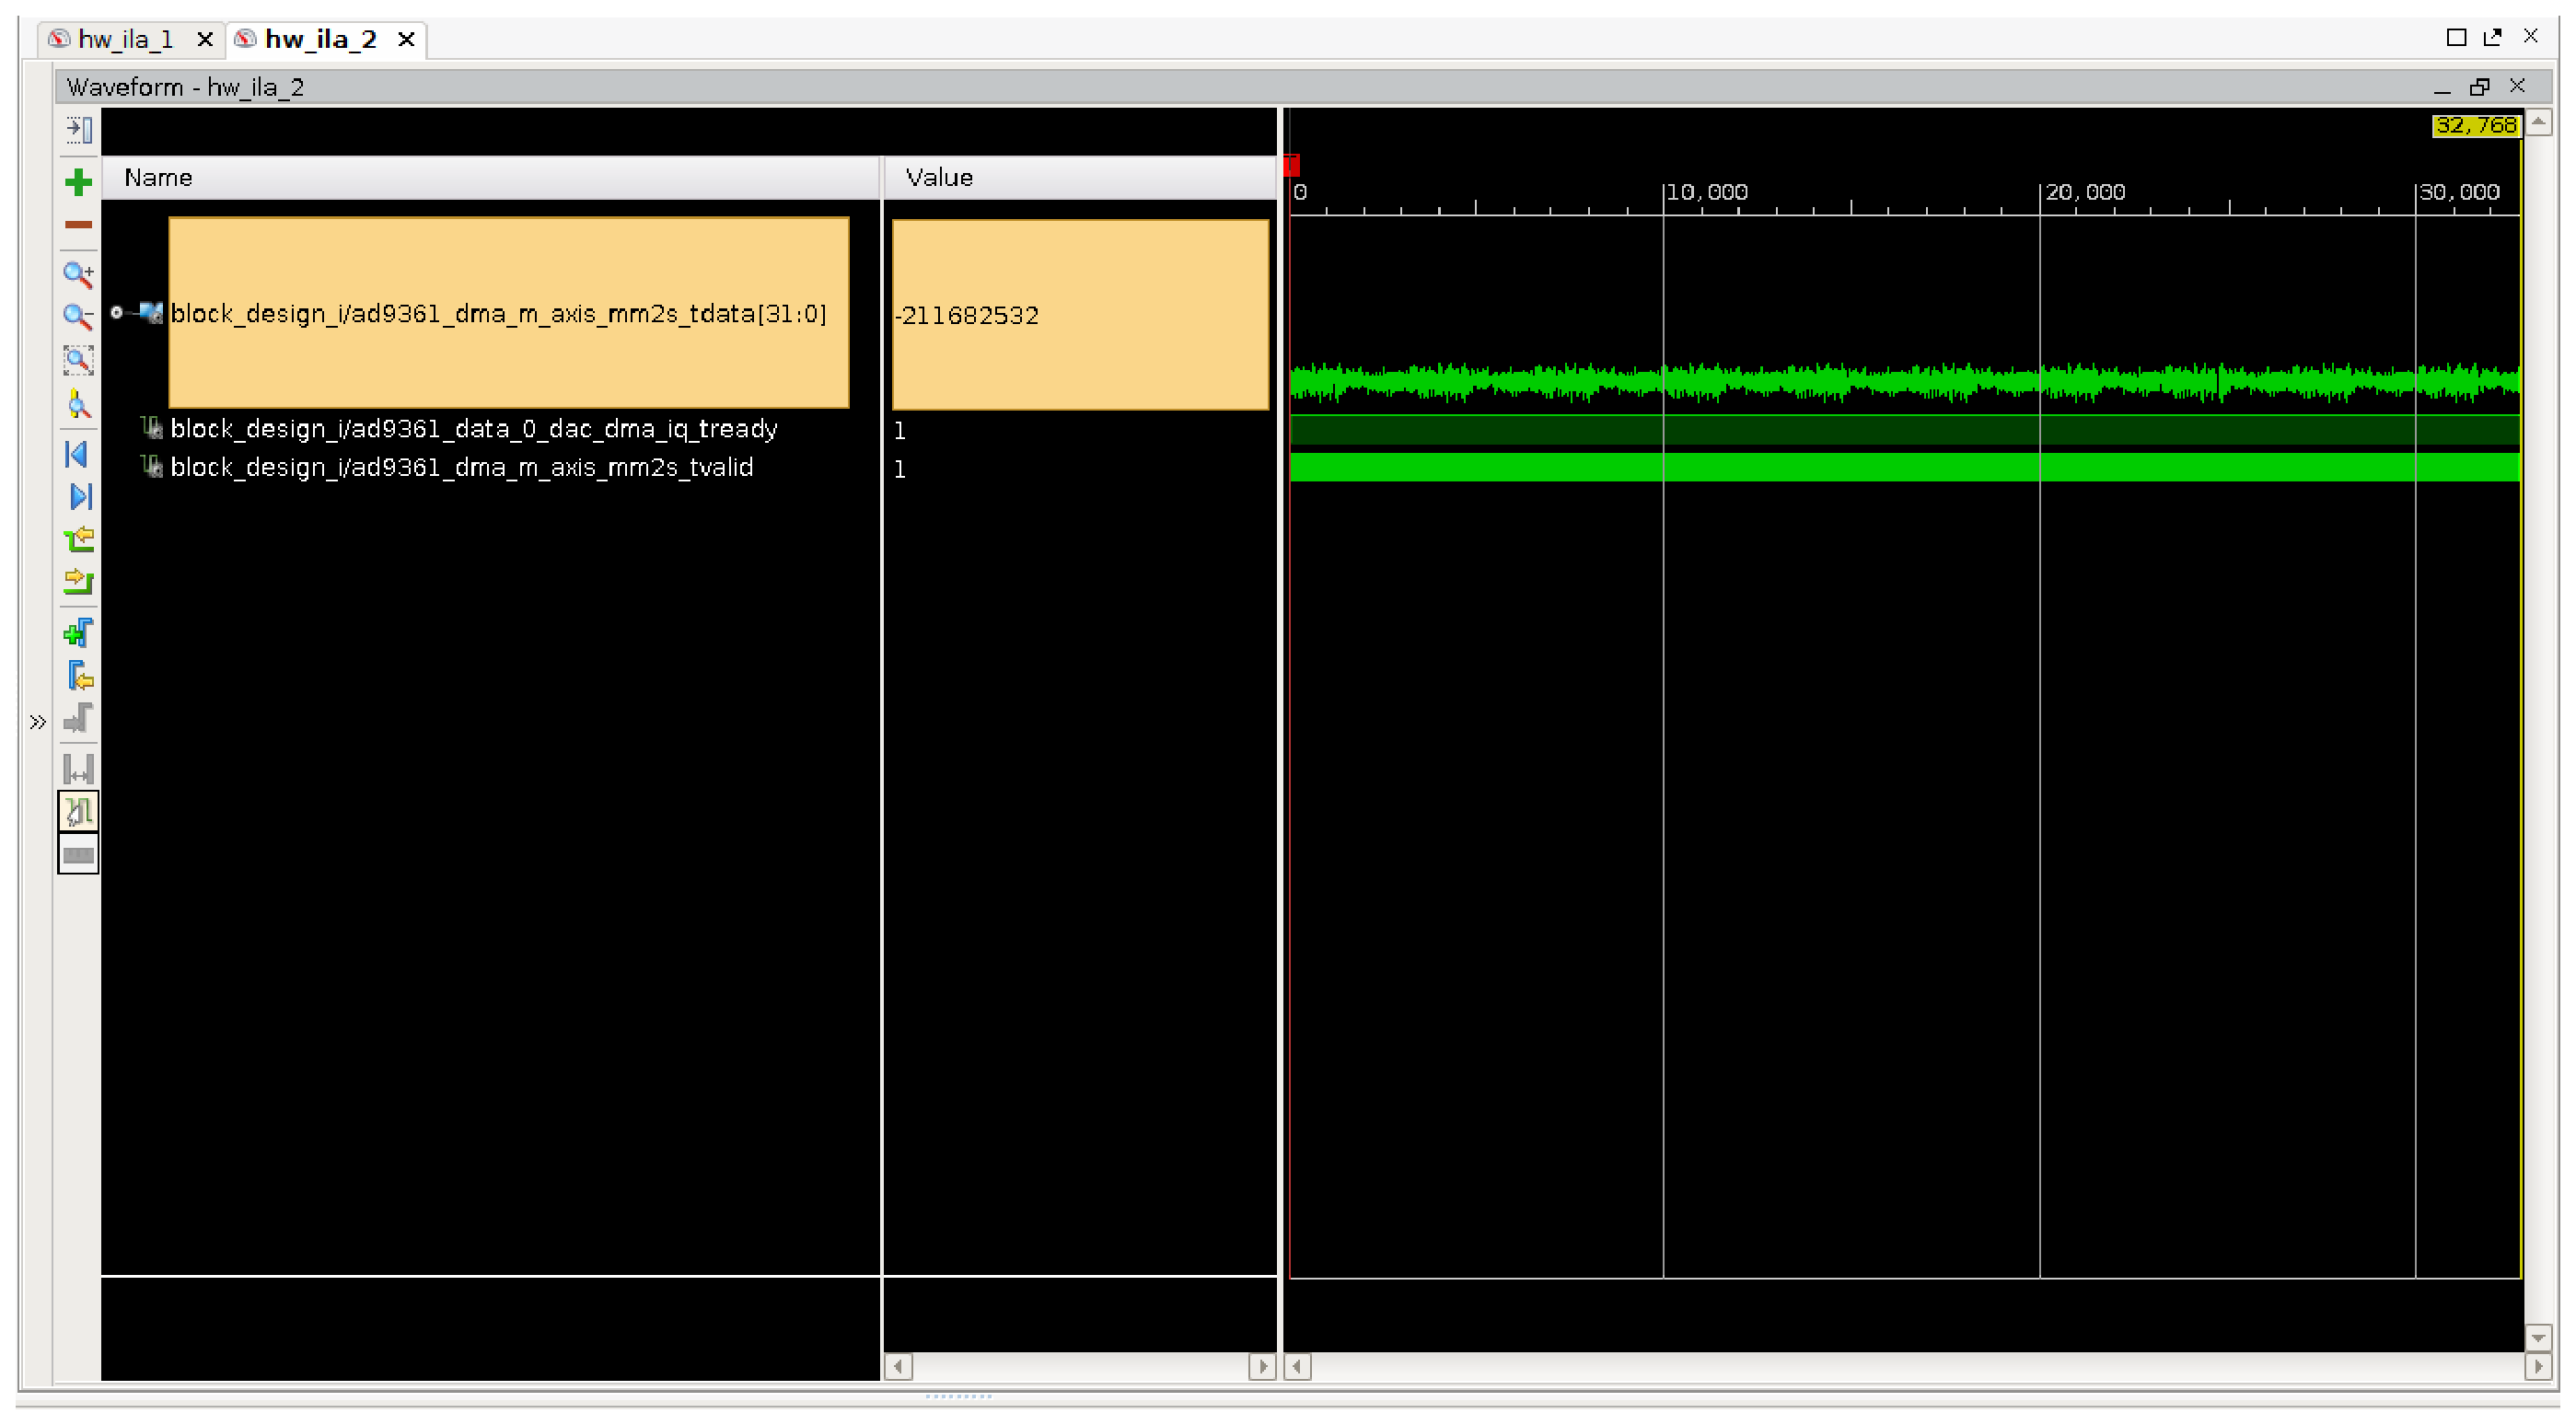
\includegraphics[width=1\textwidth,
    trim={{.11\textwidth} {.95\textwidth} {.04\textwidth} {.15\textwidth}},
    clip]{./figures/ltedac_ila}
    \caption{ Analog form data read form memory by DMA.
    \label{fig:dataflowana}}
\end{figure}

\begin{figure}[htbp]
    \centering
    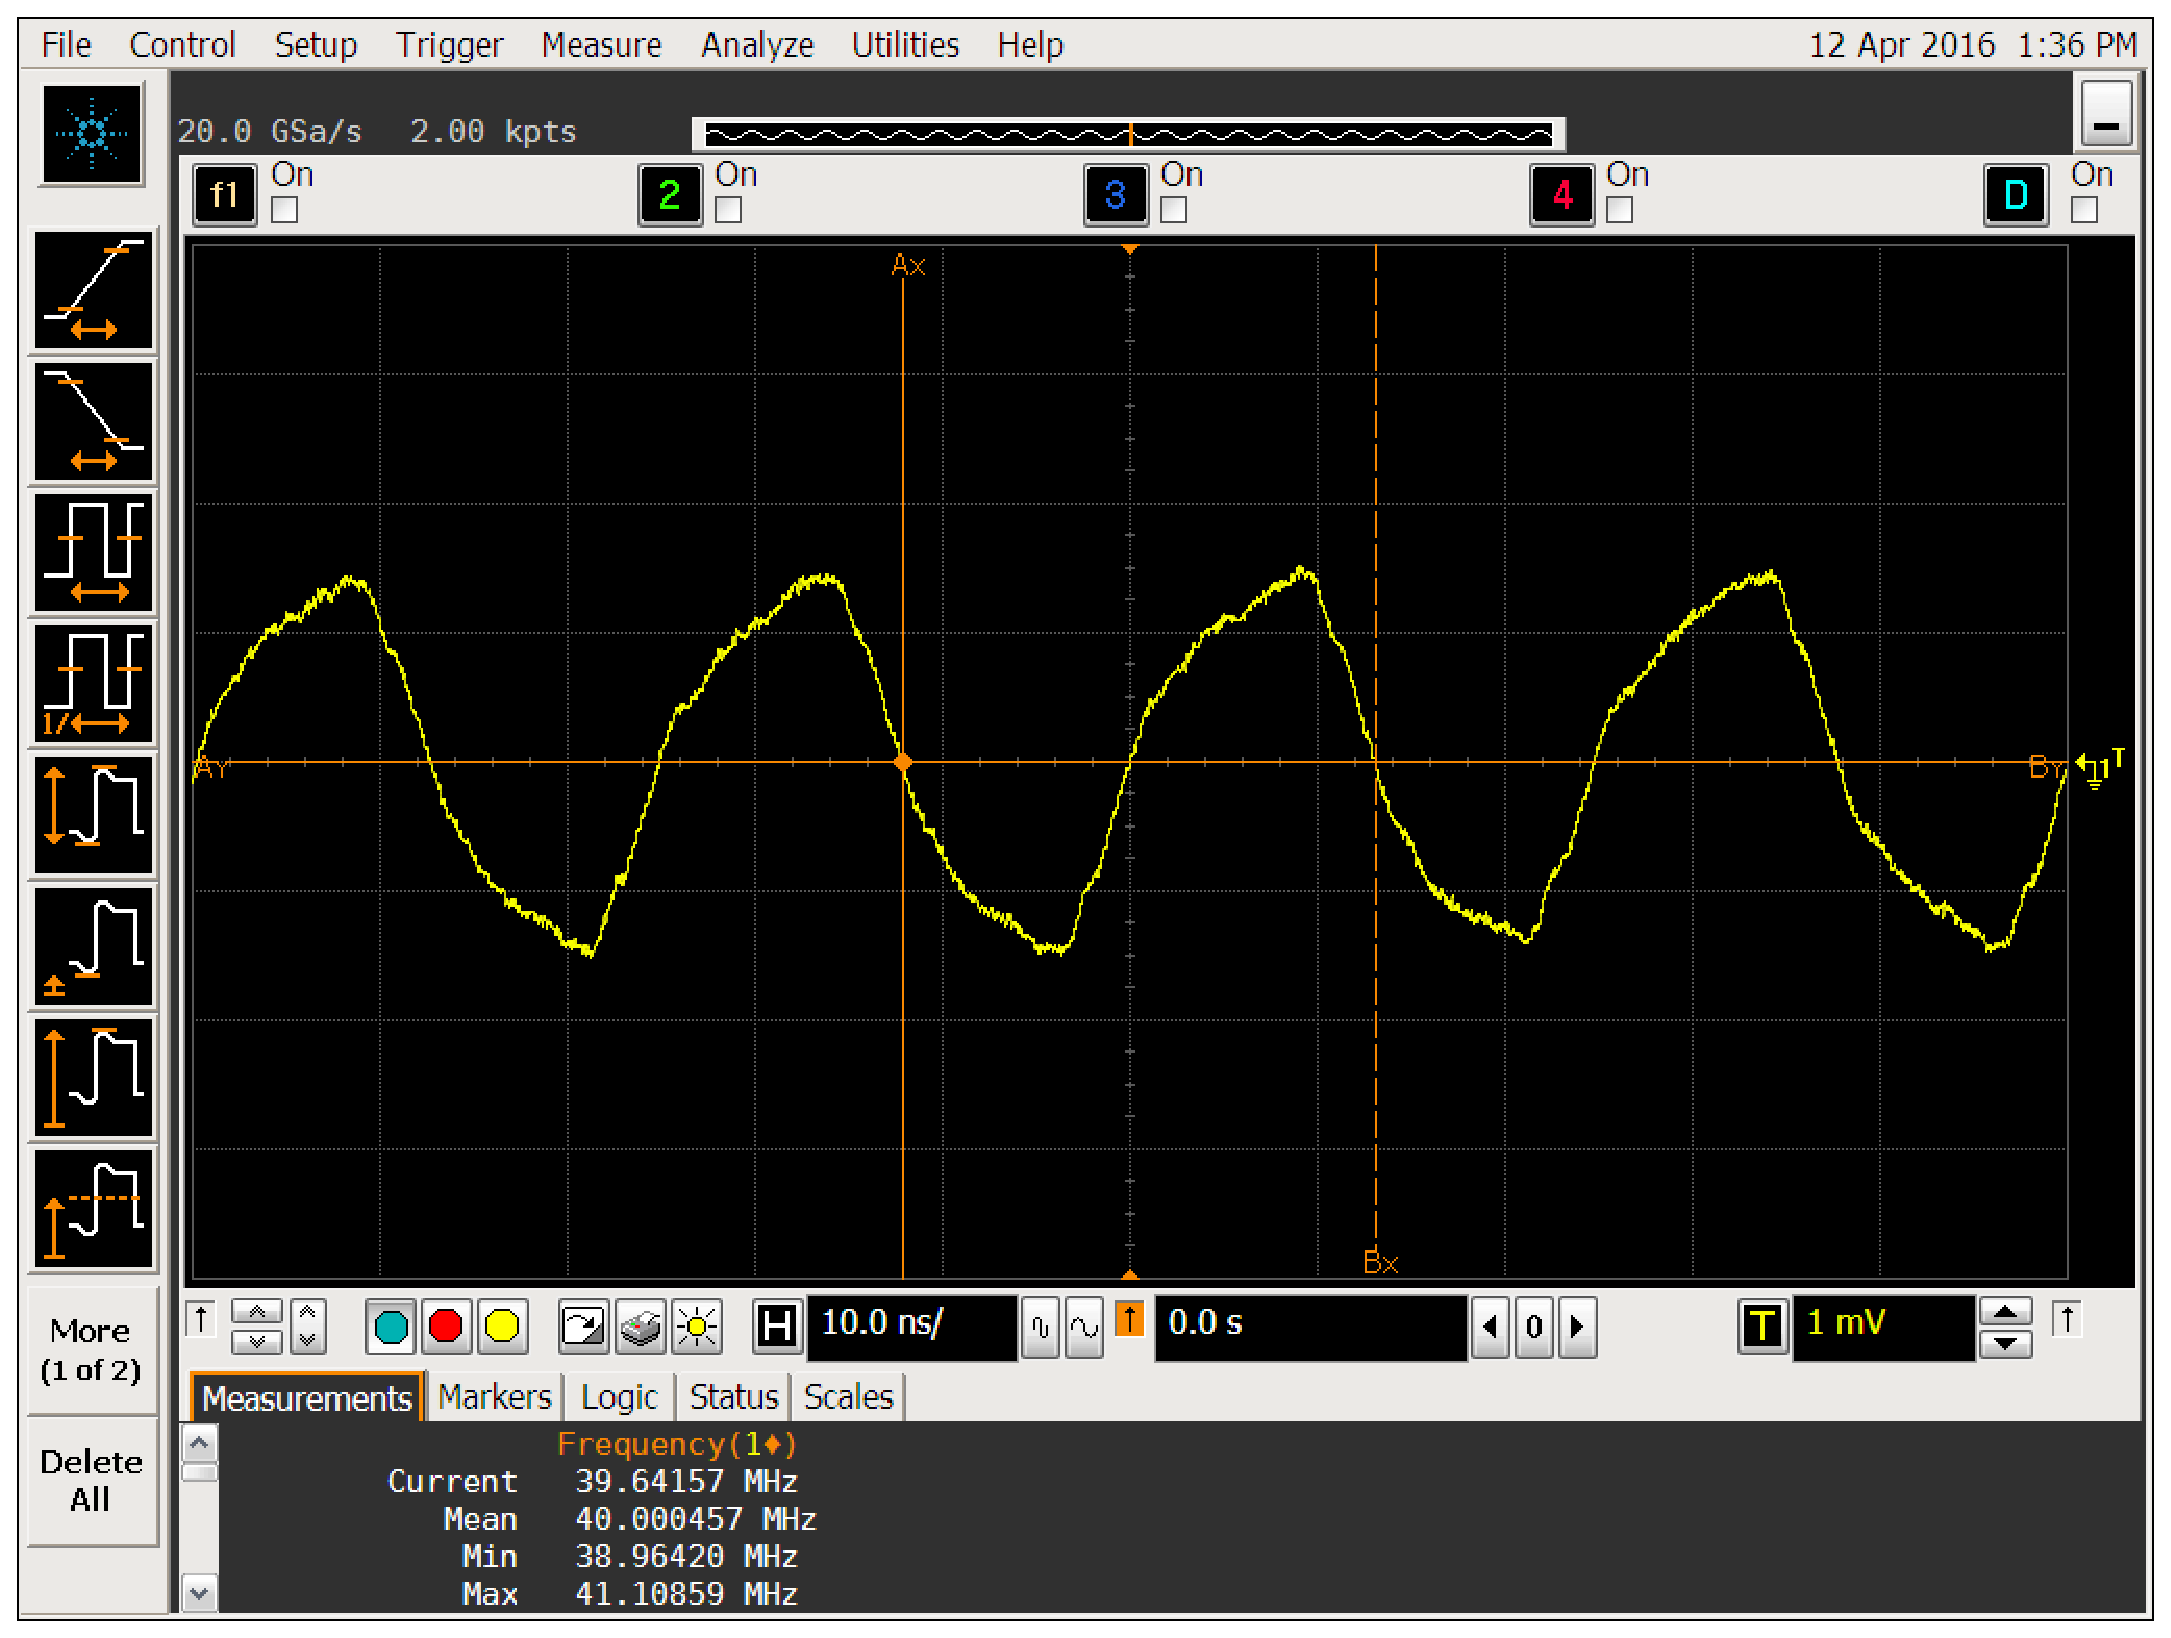
\includegraphics[width=0.85\textwidth,
    trim={{.17\textwidth} 0 {.02\textwidth} {.24\textwidth}},
    clip]{./figures/oscill_ad9361_dac_clk}
    \caption{ DAC clock output.
    \label{fig:dacclk}}
\end{figure}

\begin{figure}[htbp]
    \centering
    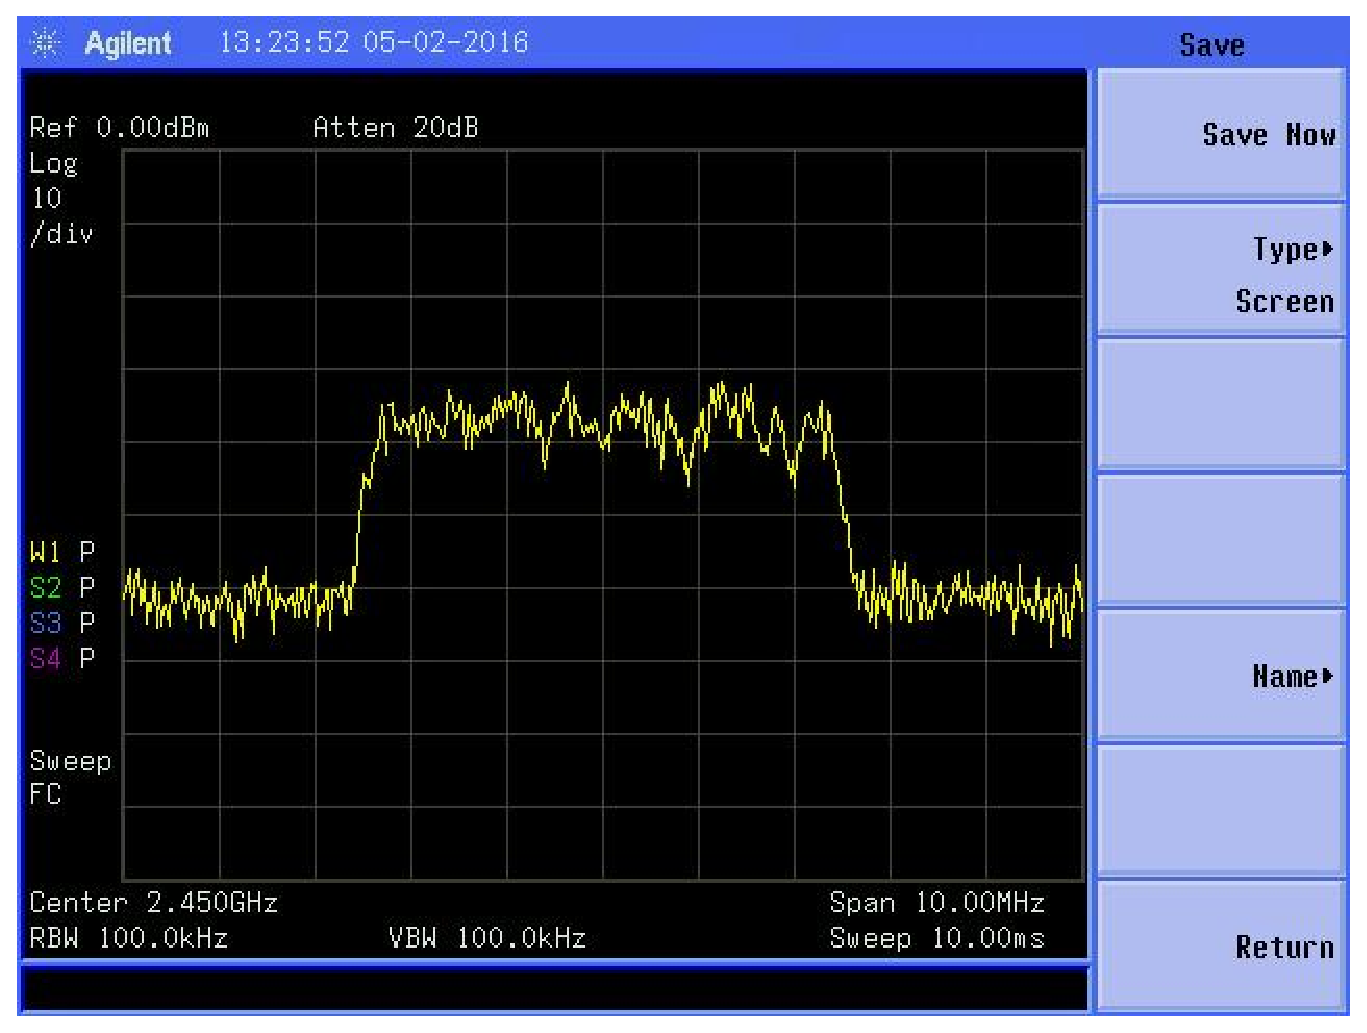
\includegraphics[width=0.8\textwidth,
    trim={0 0 {.27\textwidth} {.1\textwidth}},
    clip]{./figures/lte_5m}
    \caption{ LTE signal output from FMCOMMS2 spectrum.
    \label{fig:lte5m}}
\end{figure}

%\section{Reception Tests (ADC)}
%\label{result:adc}
%
\begin{figure}[htbp]
    \centering
    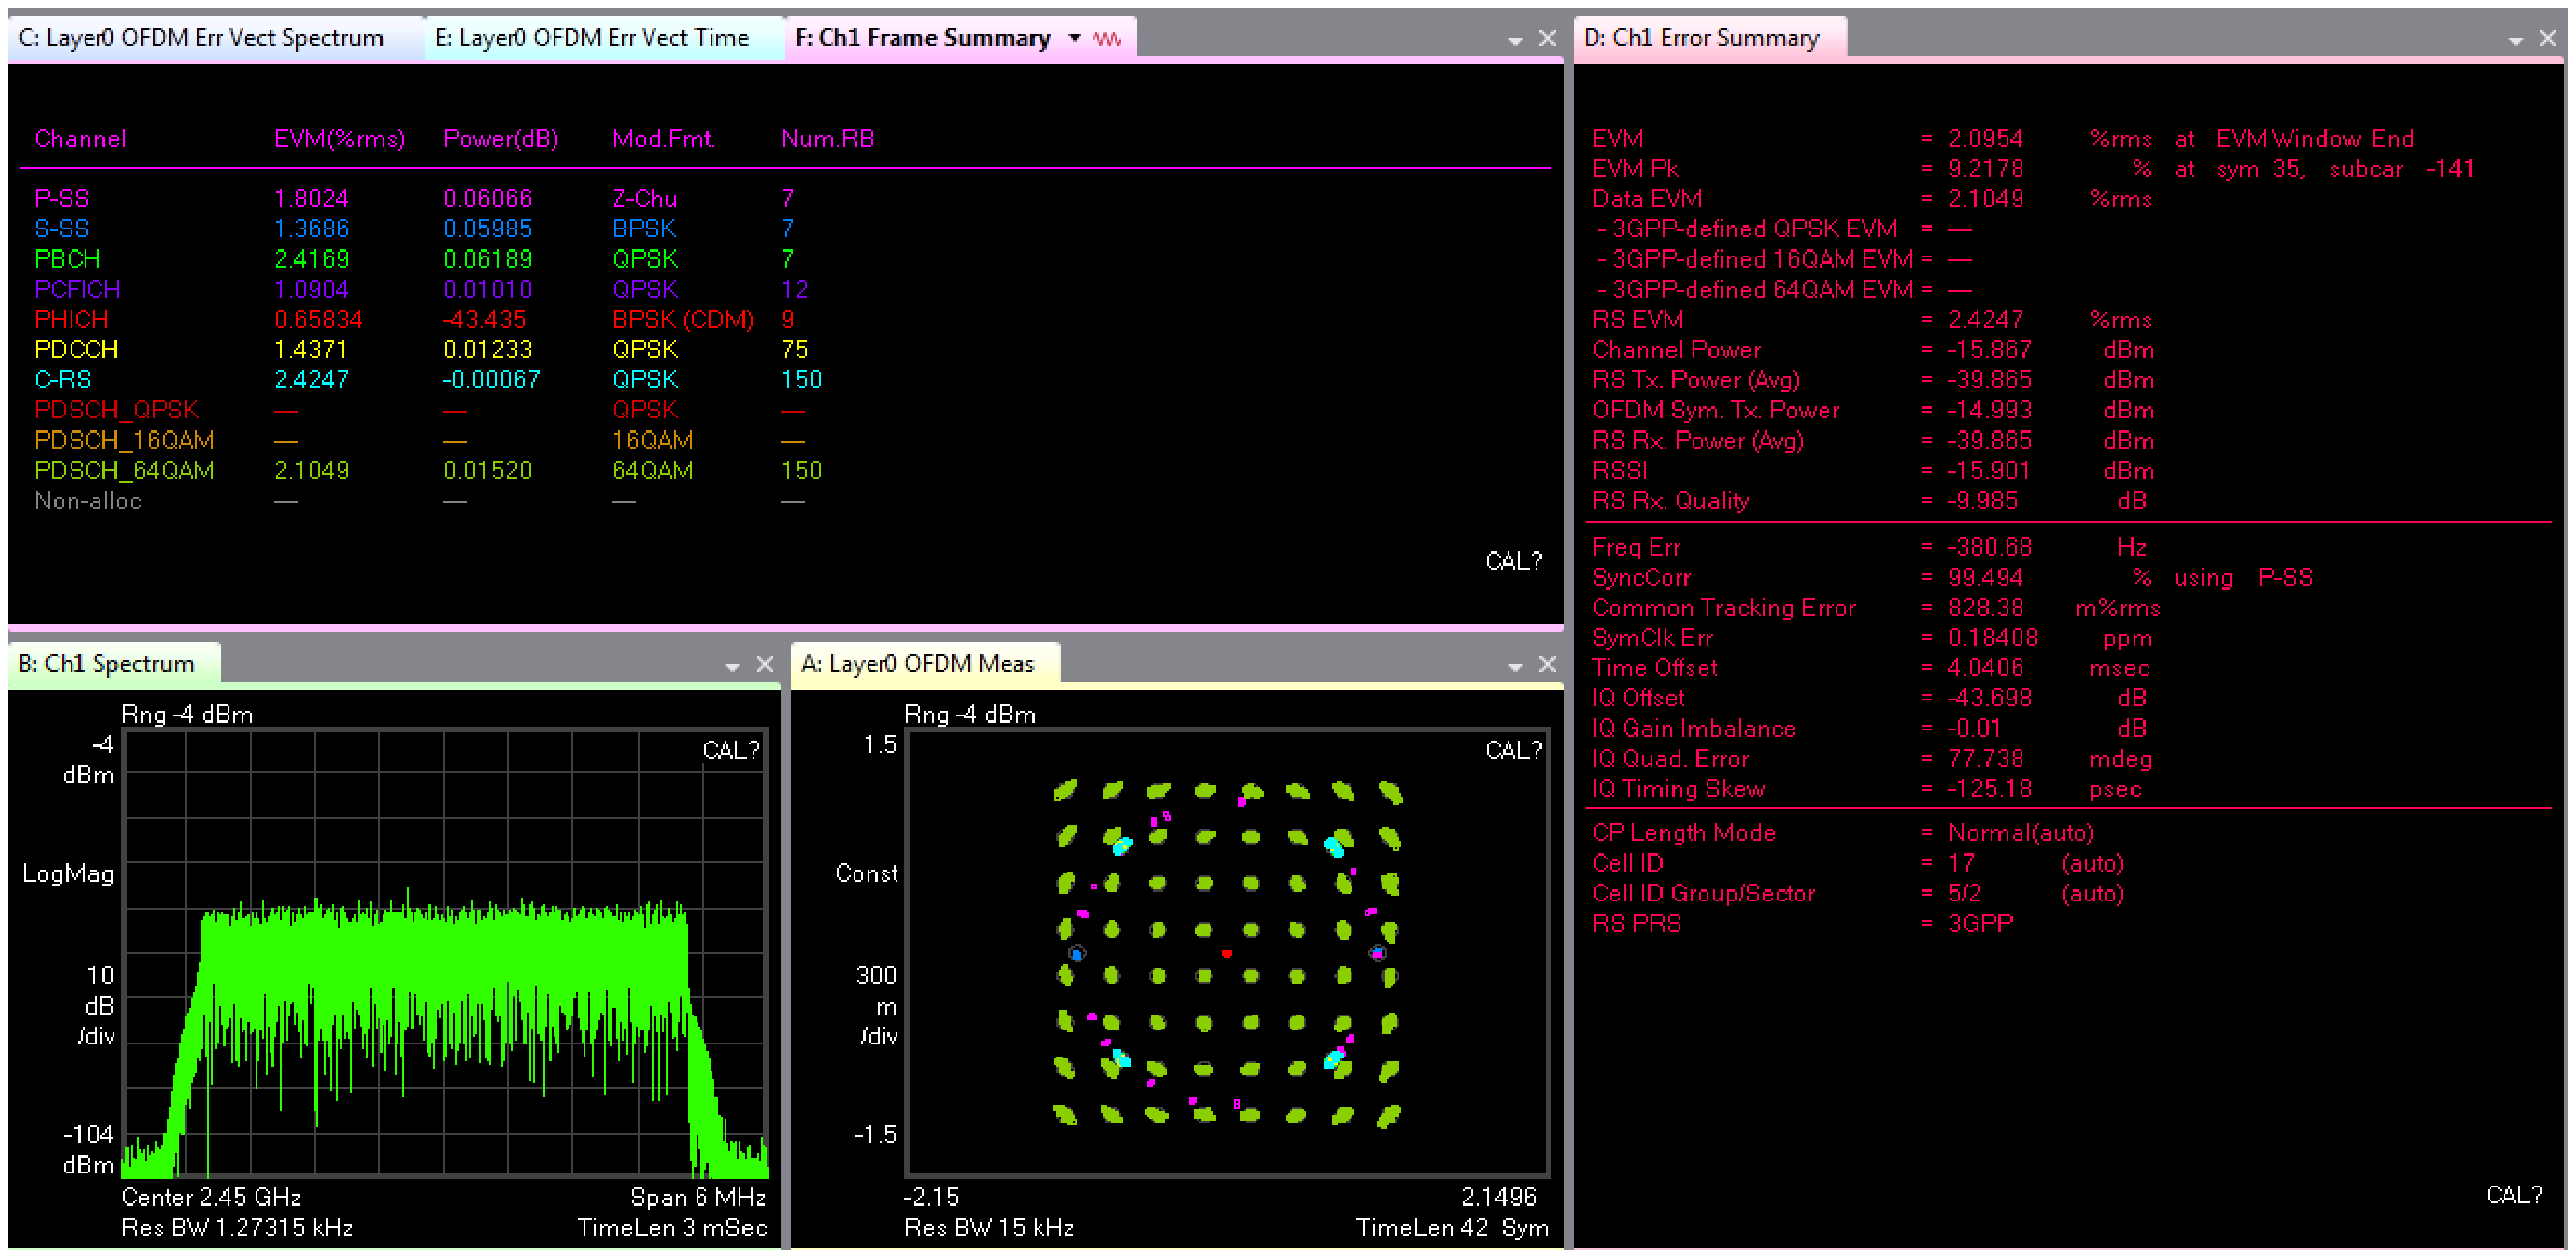
\includegraphics[width=0.95\textwidth]{./figures/evm}
    \caption{ Downlink LTE EVM.
    \label{fig:evm}}
\end{figure}
%
\vfill
\clearpage

\section{Expected Results}
\label{result:optimum}

The expected transmission of LTE signals are below demonstrated by the Analog
Devices in a LTE transmission and reception example using the same
transceiver in \cite{web:lteexamplewiki}. Comparing these results with the ones
obtained in Figure \ref{fig:evm} it is possible to note that they are similar
although both are not optimal results.

\begin{figure}[htbp]
    \centering
    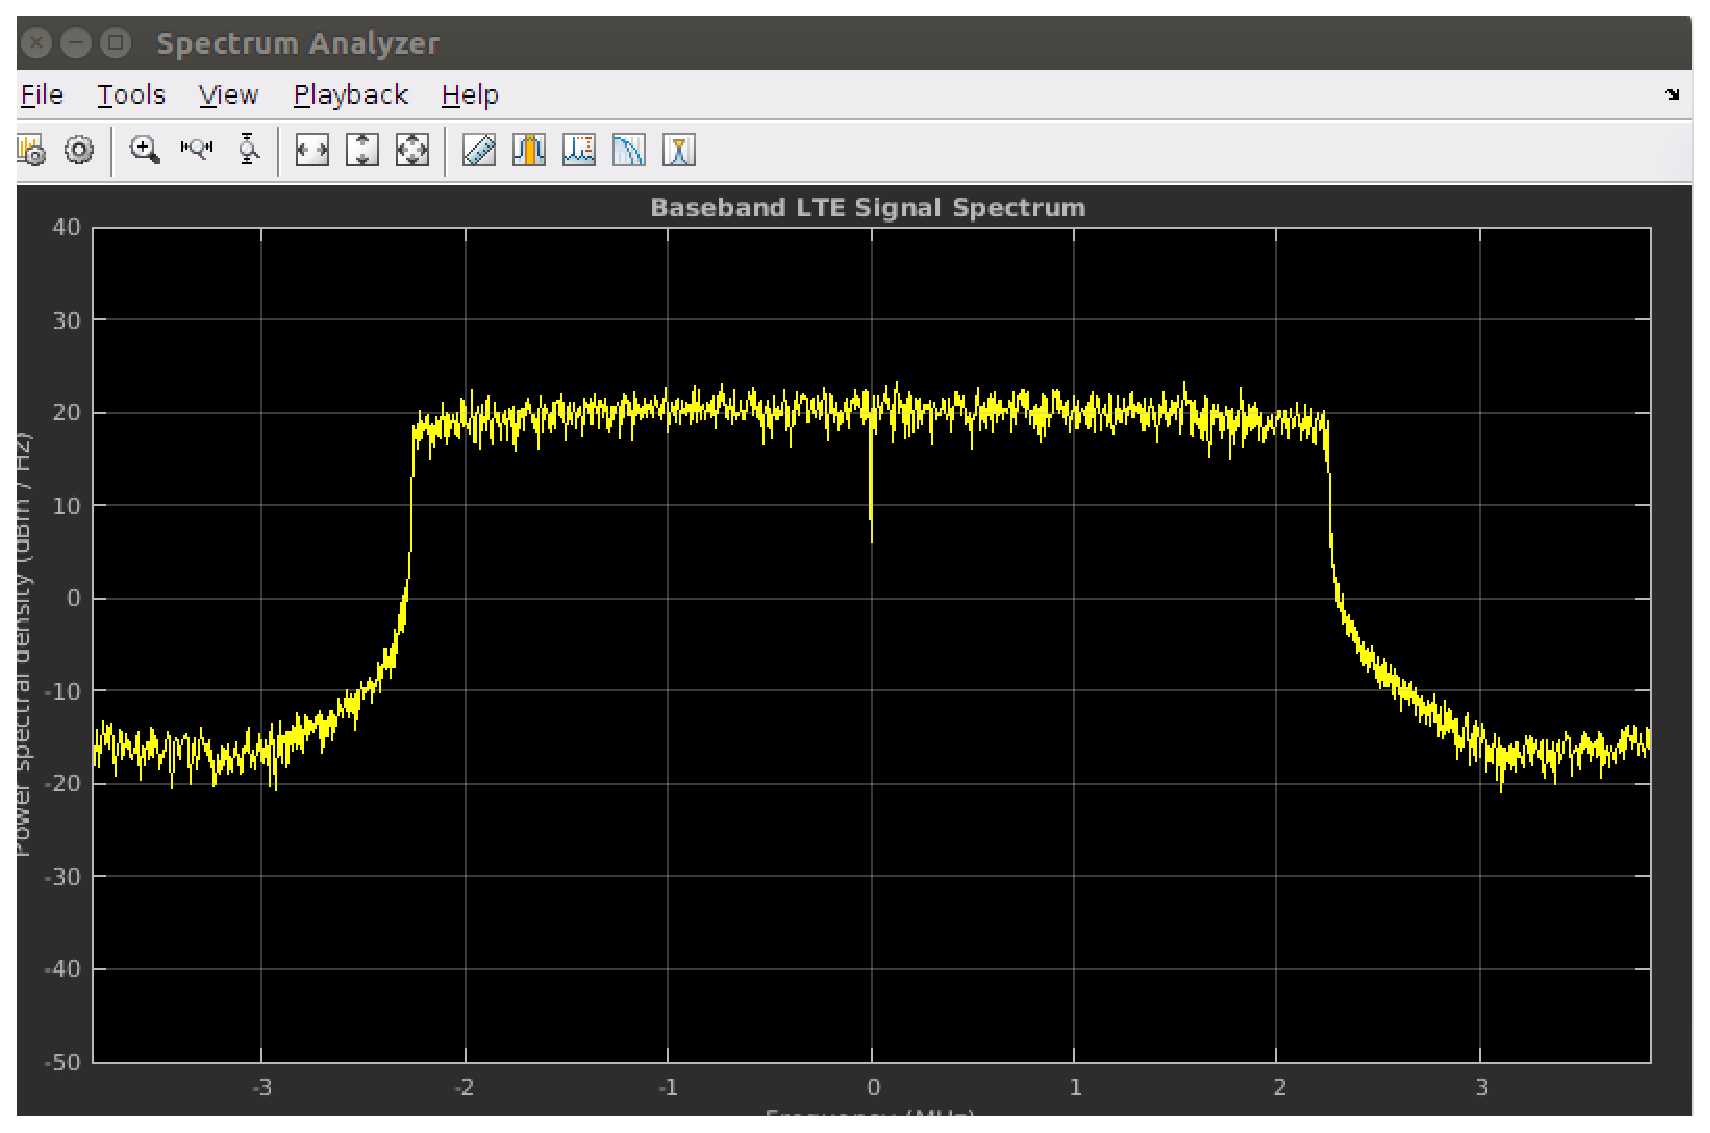
\includegraphics[width=0.65\textwidth]{./figures/lte_spectrum_iio}
    \caption{ LTE spectrum.
    \label{fig:ltespectrumiio}}
\end{figure}

\begin{figure}[htbp]
    \centering
    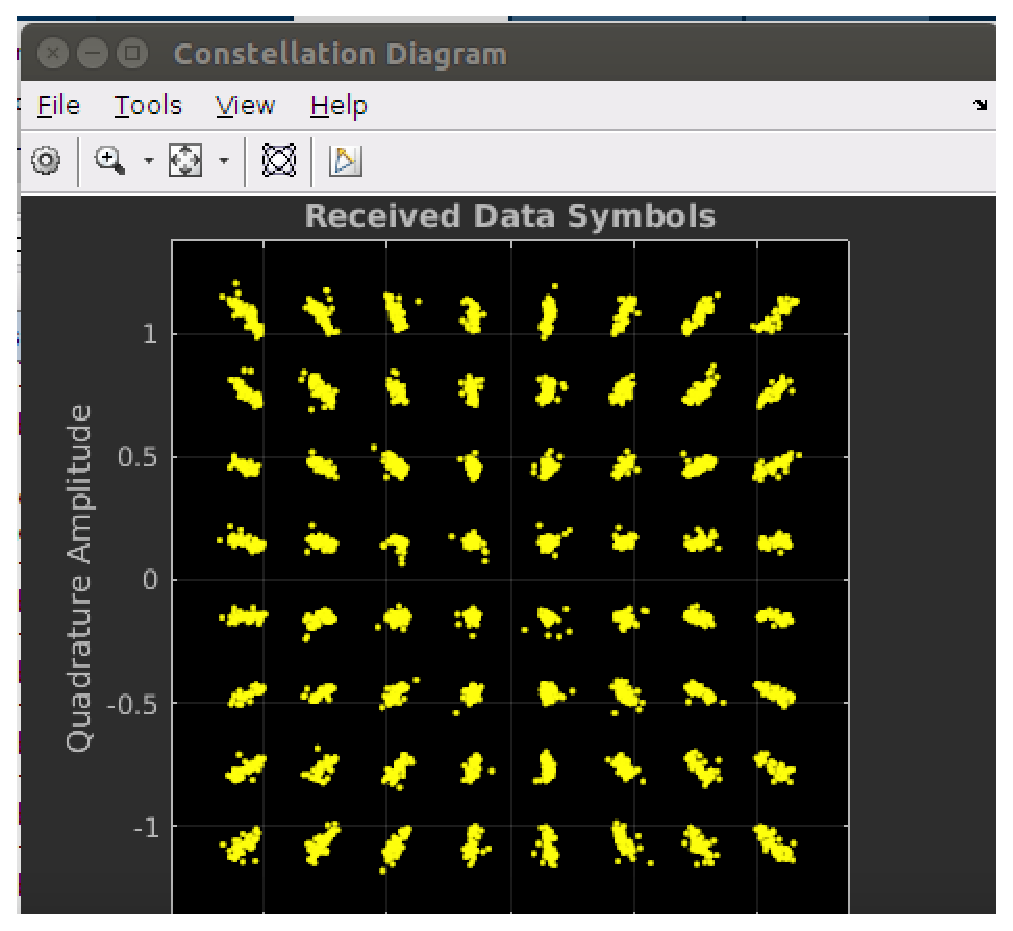
\includegraphics[width=0.55\textwidth]{./figures/lte_constellation_iio}
    \caption{ LTE constellation.
    \label{fig:lteconstellationiio}}
\end{figure}

\begin{figure}[htbp]
    \centering
    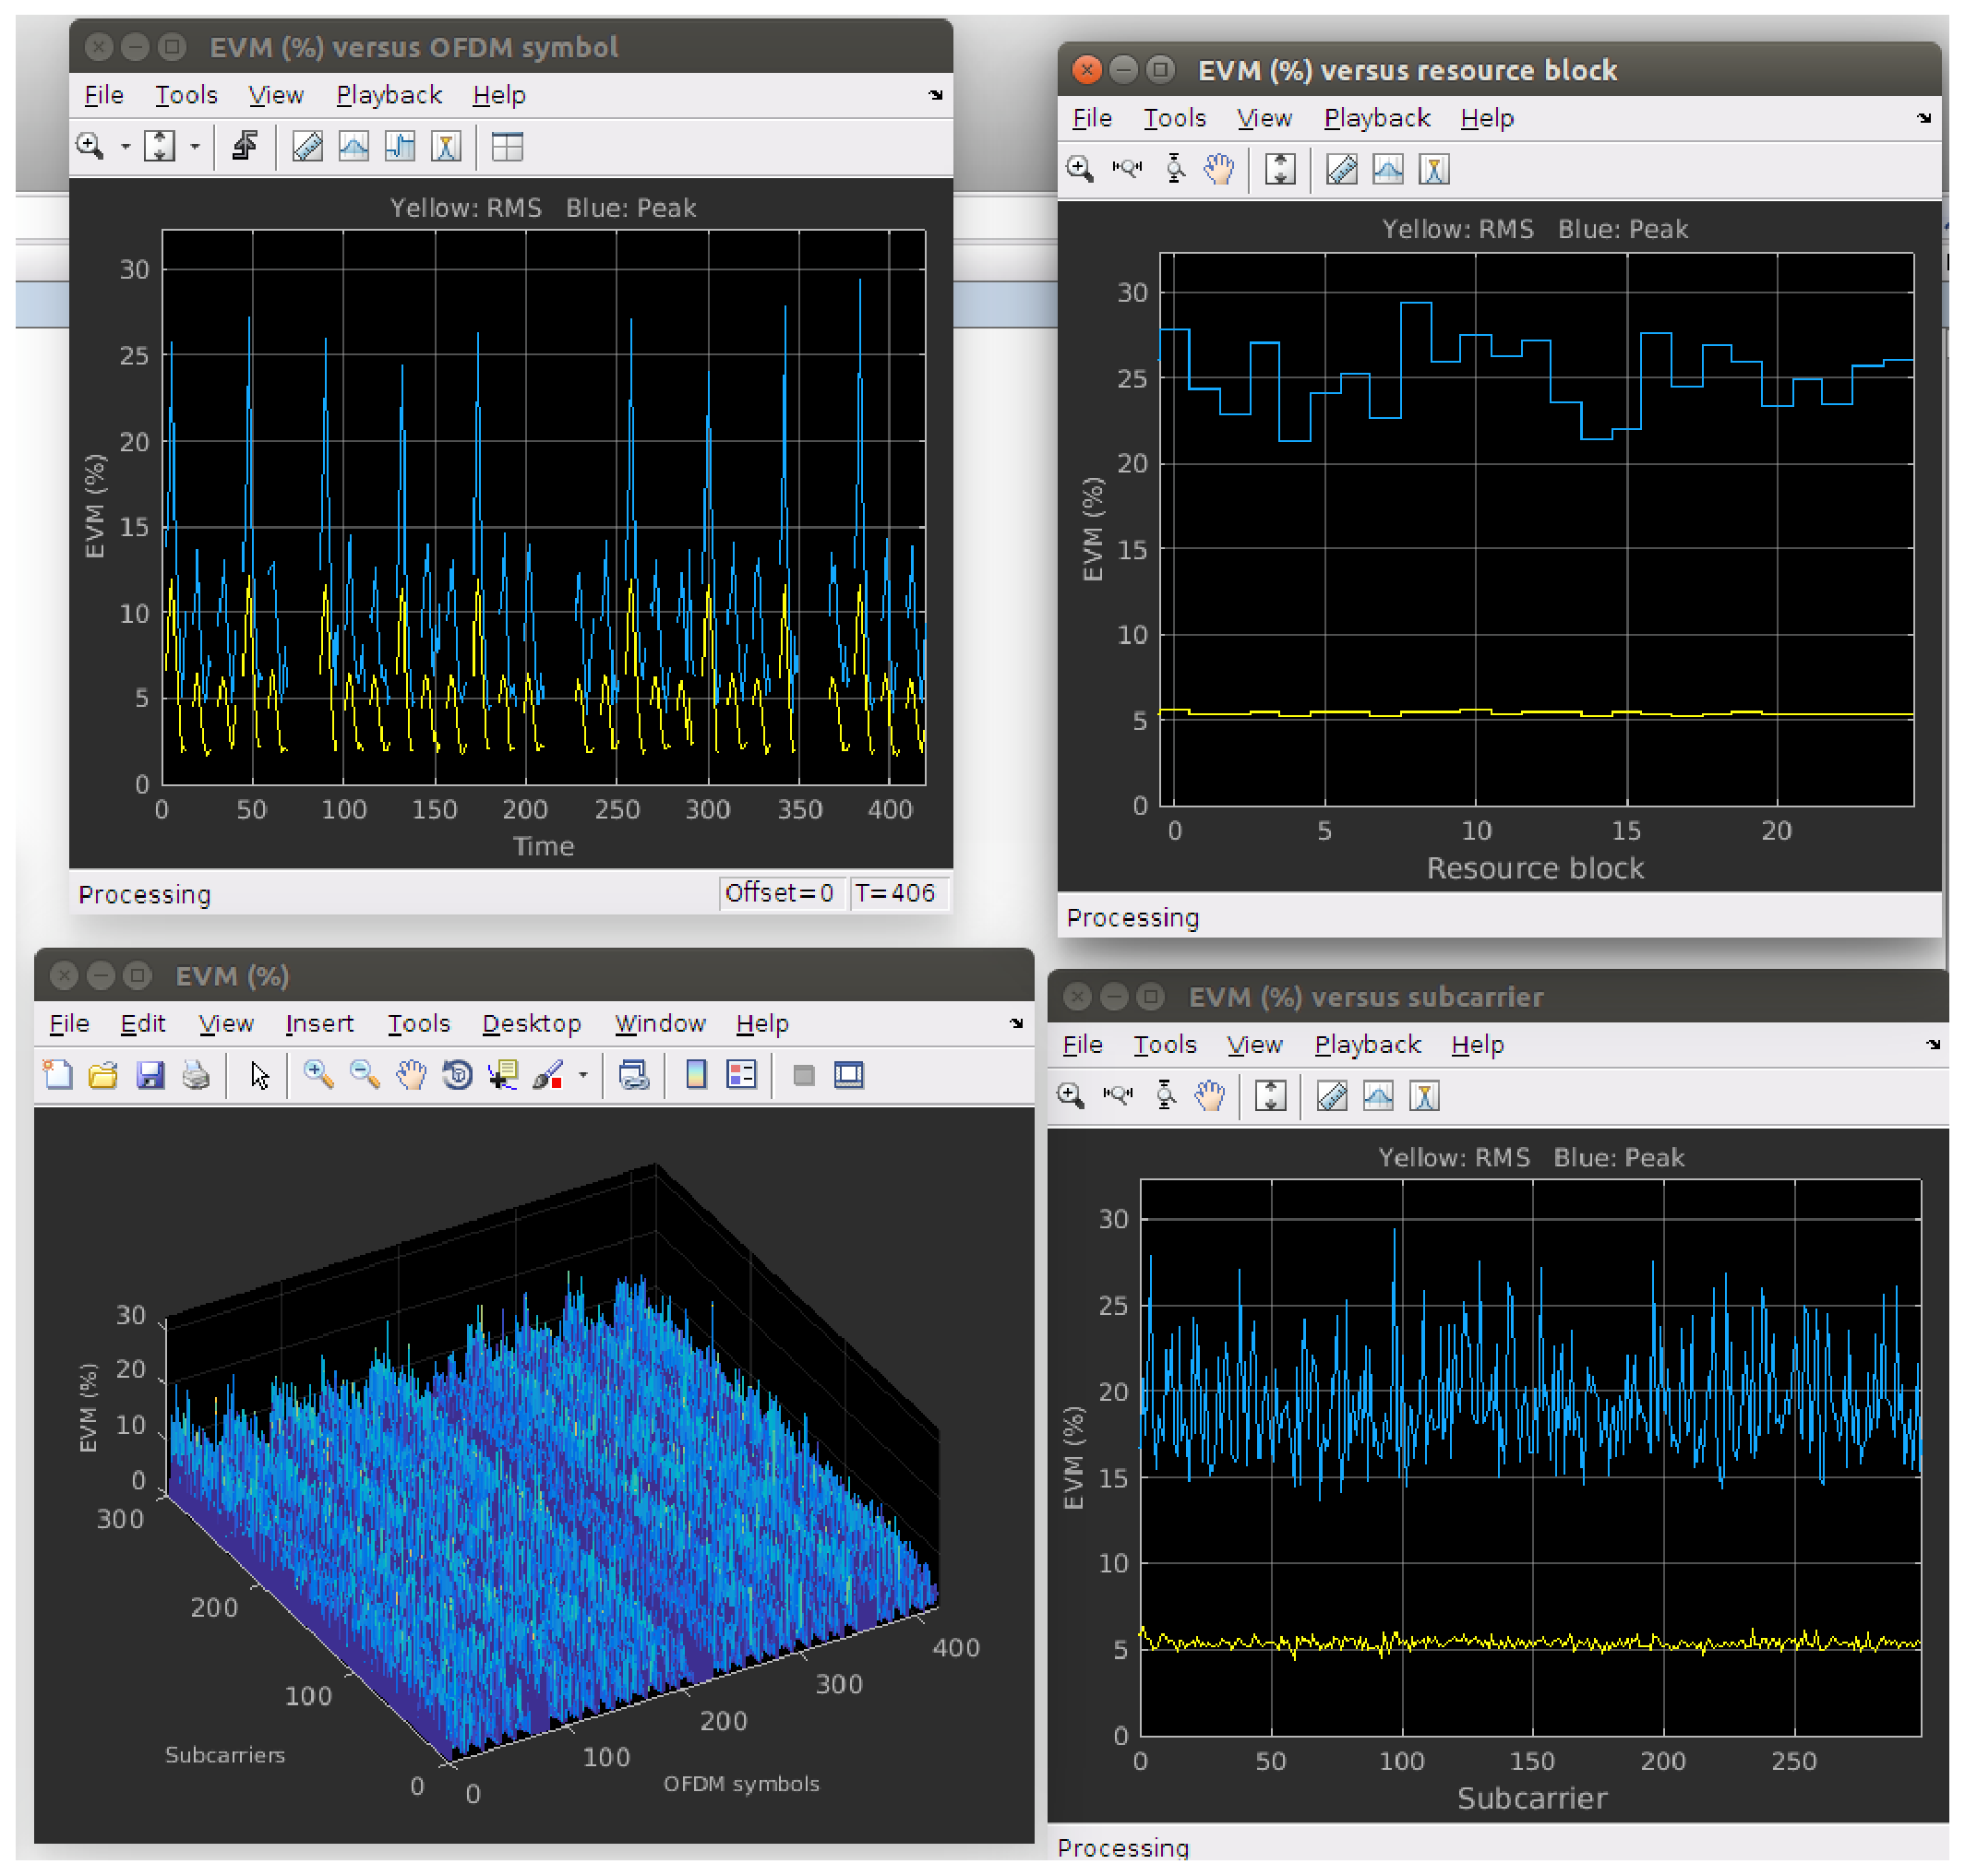
\includegraphics[width=0.85\textwidth]{./figures/lte_evm_iio}
    \caption{ LTE EVM.
    \label{fig:lteevmiio}}
\end{figure}

\vfill
\clearpage
